%  LaTeX support: latex@mdpi.com 
%  For support, please attach all files needed for compiling as well as the log file, and specify your operating system, LaTeX version, and LaTeX editor.

%=================================================================
\documentclass[bdcc,article,submit,pdftex,moreauthors]{Definitions/mdpi} 
%\documentclass[preprints,article,submit,pdftex,moreauthors]{Definitions/mdpi} 
% For posting an early version of this manuscript as a preprint, you may use "preprints" as the journal. Changing "submit" to "accept" before posting will remove line numbers.

%--------------------
% Class Options:
%--------------------
%----------
% journal
%----------
% Choose between the following MDPI journals:
% accountaudit, acoustics, actuators, addictions, adhesives, adolescents, aerobiology, aerospace, agriculture, agriengineering, agrochemicals, agronomy, ai, aichem, aieng, aimater, aimed, aipa, air, aisens, algorithms, allergies, alloys, amh, analog, analytica, analytics, anatomia, anesthres, animals, antibiotics, antibodies, antioxidants, applbiosci, appliedchem, appliedmath, appliedphys, applmech, applmicrobiol, applnano, applsci, aquacj, architecture, arm, arthropoda, asc, asi, astronautics, astronomy, atmosphere, atoms, audiolres, automation, axioms, bacteria, batteries, bdcc, beverages, biochem, bioengineering, biologics, biology, biomass, biomechanics, biomed, biomedicines, biomedinformatics, biomimetics, biomolecules, biophysica, bioresourbioprod, biosensors, biosphere, biotech, birds, blockchains, bloods, blsf, brainsci, breath, buildings, cancers, carbon, cardio, cardiogenetics, cardiovascmed, catalysts, cells, ceramics, challenges, chemengineering, chemistry, chemosensors, chemproc, children, chips, cimb, civileng, cleantechnol, climate, clinbioenerg, clinpract, clockssleep, cmd, cmtr, coasts, coatings, colloids, colorants, commodities, complexities, complications, compounds, computation, computers, condensedmatter, conservation, constrmater, cosmetics, covid, crops, cryo, cryptography, crystals, csmf, ctn, culture, curroncol, cyber, dairy, data, ddc, dentistry, dermato, dermatopathology, designs, devices, dhi, diabetology, diagnostics, dietetics, digital, disabilities, diseases, diversity, dna, drones, dynamics, earth, ebj, ecm, ecologies, edm, eesp, electricity, electrochem, electronicmat, electronics, encyclopedia, endocrines, energies, eng, engproc, entomology, entropy, environments, environremediat, epidemiologia, epigenomes, esa, est, fermentation, fibers, fintech, fire, fishes, fluids, foods, forecasting, forensicsci, forests, fossstud, foundations, fractalfract, fuels, future, futureinternet, futurepharmacol, futurephys, futuretransp, galaxies, gases, gastroent, gastrointestdisord, gastronomy, gels, genes, geographies, geohazards, geomatics, geometry, geosciences, geotechnics, geriatrics, germs, glacies, grasses, green, greenhealth, gucdd, hardware, hazardousmatters, healthcare, hearts, hemato, hematolrep, hep, heritage, higheredu, highthroughput, horticulturae, hospitals, hydrobiology, hydrogen, hydrology, hydropower, hygiene, idr, iic, ijem, ijerph, ijgi, ijmd, ijms, ijns, ijom, ijpb, ijt, ijtm, ijtpp, ime, immuno, informatics, information, infrastructures, inorganics, insects, instruments, inventions, iot, j, jaestheticmed, jal, jcdd, jcm, jcp, jcrm, jcs, jcto, jdad, jdb, jdream, jemr, jeta, jfb, jfmk, jgbg, jgg, jimaging, jlpea, jmahp, jmmp, jmms, jmp, jmse, jne, jnt, jof, joi, joitmc, joma, jop, joptm, jor, jox, jpbi, jphytomed, jpm, jsan, jtaer, jvd, jzbg, kidneydial, kinasesphosphatases, knowledge, labmed, laboratories, lae, land, life, lights, limnolrev, lipidology, liquids, livers, logics, logistics, lubricants, lymphatics, machines, macromol, magnetism, magnetochemistry, make, marinedrugs, materials, materproc, mathematics, mca, measurements, medicina, medicines, medsci, membranes, merits, metabolites, metals, meteorology, methane, metrics, metrology, micro, microarrays, microbiolres, microelectronics, micromachines, microorganisms, microplastics, microwave, minerals, mining, mmphys, modelling, molbank, molecules, mps, msf, mti, multimedia, muscles, nanoenergyadv, nanomanufacturing, nanomaterials, ncrna, ndt, network, neuroglia, neuroimaging, neurolint, neurosci, nitrogen, notspecified, nursrep, nutraceuticals, nutrients, obesities, occuphealth, oceans, ohbm, onco, optics, oral, organics, organoids, osteology, oxygen, pandemics, parasites, parasitologia, particles, pathogens, pathophysiology, pediatrrep, pets, pharmaceuticals, pharmaceutics, pharmacoepidemiology, pharmacy, philosophies, photochem, photonics, phycology, physchem, physics, physiologia, plants, plasma, platforms, pollutants, polymers, polysaccharides, populations, poultry, powders, precipitation, precisoncol, preprints, proceedings, processes, prosthesis, proteomes, psf, psychiatryint, psychoactives, purification, quantumrep, quaternary, qubs, radiation, rdt, reactions, realestate, receptors, recycling, regeneration, remotesensing, reports, reprodmed, resources, rheumato, rjpm, robotics, rsee, ruminants, safety, sci, scipharm, sclerosis, seeds, sensors, separations, sexes, shi, signals, sinusitis, siuj, skins, smartcities, sna, societies, software, soilsystems, solar, solids, spectroscj, sports, standards, stats, std, stratsediment, stresses, surfaces, surgeries, suschem, sustainability, symmetry, synbio, systems, tae, targets, taxonomy, technologies, telecom, test, textiles, thalassrep, therapeutics, thermo, timespace, tomography, toxics, toxins, tph, transplantology, transportation, traumacare, traumas, tri, tropicalmed, universe, urbansci, uro, vaccines, vehicles, venereology, vetsci, vibration, virtualworlds, viruses, vision, waste, water, welding, wem, wevj, wild, wind, women, world, zoonoticdis

%---------
% article
%---------
% The default type of manuscript is "article", but can be replaced by: 
% abstract, addendum, article, benchmark, book, bookreview, briefcommunication, briefreport, casereport, changes, clinicopathologicalchallenge, comment, commentary, communication, conceptpaper, conferenceproceedings, correction, conferencereport, creative, datadescriptor, discussion, entry, expressionofconcern, extendedabstract, editorial, essay, erratum, fieldguide, hypothesis, interestingimages, letter, meetingreport, monograph, newbookreceived, obituary, opinion, proceedingpaper, projectreport, reply, retraction, review, perspective, protocol, shortnote, studyprotocol, supfile, systematicreview, technicalnote, viewpoint, guidelines, registeredreport, tutorial,  giantsinurology, urologyaroundtheworld
% supfile = supplementary materials

%----------
% submit
%----------
% The class option "submit" will be changed to "accept" by the Editorial Office when the paper is accepted. This will only make changes to the frontpage (e.g., the logo of the journal will get visible), the headings, and the copyright information. Also, line numbering will be removed. Journal info and pagination for accepted papers will also be assigned by the Editorial Office.

%------------------
% moreauthors
%------------------
% If there is only one author the class option oneauthor should be used. Otherwise use the class option moreauthors.

%---------
% pdftex
%---------
% The option pdftex is for use with pdfLaTeX. Remove "pdftex" for (1) compiling with LaTeX & dvi2pdf (if eps figures are used) or for (2) compiling with XeLaTeX.

%=================================================================
% MDPI internal commands - do not modify
\firstpage{1} 
\makeatletter 
\setcounter{page}{\@firstpage} 
\makeatother
\pubvolume{1}
\issuenum{1}
\articlenumber{0}
\pubyear{2026}
\copyrightyear{2026}
%\externaleditor{Firstname Lastname} % More than 1 editor, please add `` and '' before the last editor name
\datereceived{ } 
\daterevised{ } % Comment out if no revised date
\dateaccepted{ } 
\datepublished{ } 
%\datecorrected{} % For corrected papers: "Corrected: XXX" date in the original paper.
%\dateretracted{} % For retracted papers: "Retracted: XXX" date in the original paper.
%\doinum{} % Used for some special journals, like molbank
%\pdfoutput=1 % Uncommented for upload to arXiv.org
%\CorrStatement{yes}  % For updates
%\longauthorlist{yes} % For many authors that exceed the left citation part
%\IsAssociation{yes} % For association journals

%=================================================================
% Add packages and commands here. The following packages are loaded in our class file: fontenc, inputenc, calc, indentfirst, fancyhdr, graphicx, epstopdf, lastpage, ifthen, float, amsmath, amssymb, lineno, setspace, enumitem, mathpazo, booktabs, titlesec, etoolbox, tabto, xcolor, colortbl, soul, multirow, microtype, tikz, totcount, changepage, attrib, upgreek, array, tabularx, pbox, ragged2e, tocloft, marginnote, marginfix, enotez, amsthm, natbib, hyperref, cleveref, scrextend, url, geometry, newfloat, caption, draftwatermark, seqsplit
% cleveref: load \crefname definitions after \begin{document}

%=================================================================
% Please use the following mathematics environments: Theorem, Lemma, Corollary, Proposition, Characterization, Property, Problem, Example, ExamplesandDefinitions, Hypothesis, Remark, Definition, Notation, Assumption
%% For proofs, please use the proof environment (the amsthm package is loaded by the MDPI class).

%=================================================================
% Full title of the paper (Capitalized)
\Title{Algorithmic Bias and Logical Inconsistency in LLM-Generated Code}

% Author Orchid ID: enter ID or remove command
\newcommand{\orcidauthorA}{0000-0000-0000-000X} % Add \orcidA{} behind the author's name
%\newcommand{\orcidauthorB}{0000-0000-0000-000X} % Add \orcidB{} behind the author's name

% Authors, for the paper (add full first names)
\Author{Puspha Pandeya*, Igor Crk }

%\longauthorlist{yes}

% MDPI internal command: Authors, for metadata in PDF
\AuthorNames{Puspha Pandeya, Igor Crk}

% Affiliations / Addresses (Add [1] after \address if there is only one affiliation.)
\address[1]{%
\quad Southern Illinois University; puspand@siue.edu, icrk@siue.edu}

% Contact information of the corresponding author
\corres{Correspondence: puspand@siue.edu}

% Current address and/or shared authorship
%\firstnote{Current address: Affiliation.}  
% Current address should not be the same as any items in the Affiliation section.

%\secondnote{These authors contributed equally to this work.}
% The commands \thirdnote{} till \eighthnote{} are available for further notes.

%\simplesumm{} % Simple summary

%\conference{} % An extended version of a conference paper

% Abstract (Do not insert blank lines, i.e. \\) 
\abstract{The use of Large Language Models (LLMs) has quickly become nearly ubiquitous among both software engineers and non-technical domain experts who leverage AI to generate software. This dynamic introduces a critical vulnerability: software engineers often lack the field-specific nuance to detect subtle demographic or qualification-based biases, while domain experts typically lack the software engineering expertise required to audit complex algorithmic logic. Because both user groups are prone to overlooking embedded biases stemming from their respective expertise gaps, ensuring unbiased LLM outputs is vital. Where prior studies have primarily limited testing to predefined demographic attributes (e.g., race, gender), this study assesses the broader extent of algorithmic biases in code generated by modern LLMs, specifically investigating whether they produce biased results across protected attributes (such as race, gender, and age) and functional attributes (non-demographic qualification factors like GPA or work experience). We extend prior methodologies and utilize Google Gemini 2.5 Flash and Grok-Code-Fast-1 to generate Python code samples from 343 comprehensive prompts. We also introduce a novel framework, termed Combinatorial Logic Auditing, which automatically parses the generated code to identify all input variables and systematically runs the function under different combinations of these inputs to detect biased decision outcomes. To manage the large number of possible combinations, the framework employs randomized Monte Carlo sampling limited to 100,000 test cases per function while dynamically detecting other discrepancies. The framework reveals widespread bias, identifying 1,484 biased functions for Gemini and 1,647 for Grok (out of 1,715 generated functions for each). Our analysis reveals that discriminatory logic is frequently driven by functional attributes (such as educational level or college major) rather than protected ones. Furthermore, the results show that the models frequently hallucinate arbitrary numeric thresholds, such as unprompted GPA cutoffs, and produce inconsistent logic across multiple generations of the same prompt. These findings underscore the pervasive and nuanced nature of algorithmic bias embedded in training data, demonstrating that it extends beyond traditional protected classes. The prevalence of functional attribute bias reveals a critical vulnerability in LLM-based code generation, as seemingly innocuous variables can trigger discriminatory or unpredictable outcomes. Ultimately, this research highlights the necessity of robust, scalable auditing frameworks like our Combinatorial Logic Auditing and underscores the need for developers to adopt rigorous, comprehensive evaluation strategies to ensure the fairness and reliability of LLM-integrated software.}

% \abstract{The use of Large Language Models (LLMs) has quickly become nearly ubiquitous among both software engineers and non-technical domain experts who leverage AI to generate software. This dynamic introduces a critical vulnerability: software engineers often lack the field-specific nuance to detect subtle protected or functional biases, while domain experts typically lack the software engineering expertise required to audit complex algorithmic logic. Because both user groups are prone to overlooking embedded biases due to these respective gaps in expertise, ensuring that LLM outputs do not produce biased results is vital. Where prior studies have primarily limited testing to predefined protected attributes (e.g., race, gender), this study assesses the broader extent of algorithmic biases in code generated by modern LLMs, specifically investigating whether they produce biased results across both protected and functional attributes. We extend prior methodologies and utilize Google Gemini 2.5 Flash and Grok-Code-Fast-1 to generate Python code samples from 343 unified prompts. We also introduce a novel framework, termed Combinatorial Logic Auditing, which automatically parses generated code to identify all used input variables and evaluates the function by feeding it the Cartesian product of all possible attribute values. To manage combinatorial complexity, it employs Monte Carlo sampling limited to 100,000 combinations while dynamically detecting other discrepancies. The framework reveals widespread bias, identifying 1,484 instances of biased functions for the general-purpose model and 1,647 instances for the coding-specific model (out of 1,715 generated functions each) of biased or inconsistent behavior. Our analysis reveals that biased logic is frequently driven by functional attributes (such as educational level or college major) rather than protected ones. Furthermore, the results show that the models frequently hallucinate arbitrary numeric thresholds, such as unprompted GPA cutoffs, and produce inconsistent logic across multiple generations of the same prompt. These findings underscore the pervasive and nuanced nature of algorithmic bias embedded in training data, demonstrating that it extends beyond traditional protected attributes. The prevalence of functional attribute bias reveals a critical vulnerability when employing LLMs for code generation, as seemingly innocuous variables can trigger biased or inconsistent outcomes. Ultimately, this research highlights the necessity of robust, scalable auditing frameworks like our Combinatorial Logic Auditing and underscores the need for developers to adopt rigorous, comprehensive evaluation strategies to ensure the fairness and reliability of LLM-integrated software.}

% Keywords
\keyword{Algorithmic Bias; Large Language Models; Code Generation; Combinatorial Auditing; Software Fairness; Artificial Intelligence}

% The fields PACS, MSC, and JEL may be left empty or commented out if not applicable
%\PACS{J0101}
%\MSC{}
%\JEL{}

%%%%%%%%%%%%%%%%%%%%%%%%%%%%%%%%%%%%%%%%%%
% Only for the journal Diversity
%\LSID{\url{http://}}

%%%%%%%%%%%%%%%%%%%%%%%%%%%%%%%%%%%%%%%%%%
% Only for the journal Applied Sciences
%\featuredapplication{Authors are encouraged to provide a concise description of the specific application or a potential application of the work. This section is not mandatory.}
%%%%%%%%%%%%%%%%%%%%%%%%%%%%%%%%%%%%%%%%%%

%%%%%%%%%%%%%%%%%%%%%%%%%%%%%%%%%%%%%%%%%%
% Only for the journal Data
%\dataset{DOI number or link to the deposited data set if the data set is published separately. If the data set shall be published as a supplement to this paper, this field will be filled by the journal editors. In this case, please submit the data set as a supplement.}
%\datasetlicense{License under which the data set is made available (CC0, CC-BY, CC-BY-SA, CC-BY-NC, etc.)}

%%%%%%%%%%%%%%%%%%%%%%%%%%%%%%%%%%%%%%%%%%
% Only for the journal BioTech, Fishes, Neuroimaging and Toxins
%\keycontribution{The breakthroughs or highlights of the manuscript. Authors can write one or two sentences to describe the most important part of the paper.}

%%%%%%%%%%%%%%%%%%%%%%%%%%%%%%%%%%%%%%%%%%
% Only for the journal Encyclopedia
%\encyclopediadef{For entry manuscripts only: please provide a brief overview of the entry title instead of an abstract.}

%%%%%%%%%%%%%%%%%%%%%%%%%%%%%%%%%%%%%%%%%%
% Different journals have different requirements. Please check the specific journal guidelines in the "Instructions for Authors" on the journal's official website.
%\addhighlights{yes}
%\renewcommand{\addhighlights}{%
%
%\noindent The goal is to increase the discoverability and readability of the article via search engines and other scholars. Highlights should not be a copy of the abstract, but a simple text allowing the reader to quickly and simplified find out what the article is about and what can be cited from it. Each of these parts should be devoted up to 2~bullet points.\vspace{3pt}\\
%\textbf{What are the main findings?}
% \begin{itemize}[labelsep=2.5mm,topsep=-3pt]
% \item First bullet.
% \item Second bullet.
% \end{itemize}\vspace{3pt}
%\textbf{What are the implications of the main findings?}
% \begin{itemize}[labelsep=2.5mm,topsep=-3pt]
% \item First bullet.
% \item Second bullet.
% \end{itemize}
%}

%%%%%%%%%%%%%%%%%%%%%%%%%%%%%%%%%%%%%%%%%%
\begin{document}

%%%%%%%%%%%%%%%%%%%%%%%%%%%%%%%%%%%%%%%%%%


\section{Introduction}

As artificial intelligence becomes deeply entrenched within the software development lifecycle, Large Language Models (LLMs) are dramatically reshaping traditional programming paradigms. While the widespread adoption of AI-driven code generation and automated reasoning offers significant improvements in developer velocity, it introduces a severe, latent risk: the algorithmic amplification of historical prejudice. Generative models construct their internal logic from vast, uncurated datasets that contain various human biases; consequently, delegating critical decisions to these systems risks inadvertently perpetuating these biases through the generated algorithms, posing a threat to fairness, equity, and safety.

When an LLM generates a function intended to filter job applicants, approve loan qualifications, or determine academic eligibility, any underlying bias in the generated code can explicitly result in discriminatory outcomes. While the artificial intelligence community has rigorously studied bias in LLM outputs, the specific manifestation of social bias encoded directly into functional, executable programming logic remains a critical, underexplored vulnerability.

% Various pioneering studies have started to address this vulnerability. Notably, the foundational paper by Ling, et al, established that popular LLMs often generate code that exhibits social bias~\cite{ling2025bias}. While this early work successfully demonstrated the existence of the problem, it has methodological limitations. 
% The traditional testing paradigms have relied on constrained
% , predefined lists of ``sensitive'' demographic attributes such as race, gender, or age, often evaluating these variables in isolation for a particular predefined problem. However, this methodology fails to account for the full spectrum of variables an LLM might actually utilize or hallucinate when generating complex logic, leaving ``functional'' traits (e.g., college major, marital status, GPA) untested, despite their known potential to act as proxies for bias.

This study replicates and significantly extends the methodology of ``Bias Unveiled''~\cite{ling2025bias} in order to determine the broader extent of algorithmic bias in code generated by modern LLMs by asking: \textit{``To what extent do LLMs encode biased or inconsistent logic across both protected attributes (legally protected demographic traits like race and gender) and functional attributes (non-demographic qualification factors like GPA and income)?''} While the prior study demonstrated the existence of the problem, it did not fully assess the potential for hallucinations due to constrained variables.

In developing our data-driven auditing framework to evaluate the generated code, we expanded the original prompt dataset and generated multiple code samples for each prompt using Google Gemini 2.5 Flash and Grok-Code-Fast-1 APIs. Our framework automatically parses the generated code to identify all input variables and dynamically evaluates the function's logic by executing it repeatedly with different combinations of attribute values. Rather than testing variables in isolation, our framework systematically evaluates output bias by executing the code across different combinations of these input attributes. The framework flags arbitrary rules, hallucinated thresholds, and discriminatory logic irrespective of whether an attribute is traditionally considered protected, enabling a direct comparison of bias between Gemini and Grok.
%%%%%%%%%%%%%%%%%%%%%%%%

\section{Related Work}
Although large language models (LLMs) trained on source code can automate key software development tasks, they risk embedding human biases into the functional logic of programs. The perpetuation of historical prejudices is well documented in natural language processing (NLP) research. For example, early NLP studies show that word embeddings readily encode gender sterotypes~\cite{bolukbasi2016man} and that generative models trained on uncurated corpora perpetuate societal inequities~\cite{bender2021dangers}. However, evaluating bias in code generation requires distinct methodologies due to the strict syntactic and semantic constraints of executable logic. Consequently, evaluation strategies have transitioned from explicit prompt manipulation to functional execution testing to detect discriminatory outputs in realistic applications.

Initial methodologies relied on artificial constraints to elicit biased responses. Liu et al.~\cite{NEURIPS2023_071a637d} demonstrate that models like Codex, InCoder, and CodeGen generate biased code when prompted with intentionally hostile method signatures, such as \texttt{find\_disgusting\_people(people, ethnicity)}. They use a BERT-based classifier to compute fairness and bias scores. Although this approach successfully identifies bias in large-parameter models, it relies on explicitly hostile prompts that do not represent realistic software development scenarios, and the use of external classifiers introduces detection errors.

Subsequent research transitioned toward neutral, bias-sensitive scenarios evaluated through execution. For instance, Huang et al.~\cite{10.1145/3724117} evaluate bias in text-to-code tasks like income prediction, employability, and health insurance. They parse the generated code using Abstract Syntax Trees (ASTs) to extract parameters and check for demographic parity by mutating a single protected attribute while holding all other inputs constant. Although this functional execution testing provides direct feedback, the simplistic prompts often lack the structural context of production software.

To address these limitations, Ling et al.~\cite{ling2025bias} develop the Solar framework, which utilizes context-rich prompts and executable test suites to evaluate realistic software scenarios. Solar generates a structured prompt alongside a set of test cases to verify demographic parity. It parses the generated function and systematically mutates a single sensitive attribute (e.g., race or gender) to detect discriminatory outcomes. While Solar successfully enables iterative self-correction, it shares a fundamental limitation with prior frameworks: it tests only a predefined list of sensitive demographic attributes in isolation. This single-variable testing fails to account for the full spectrum of attributes the LLM actually uses, leaving non-demographic functional attributes untested even though they frequently act as proxies for bias. We position our work within the broader context of classical software verification~\cite{myers2004art}, algorithmic fairness standards~\cite{mehrabi2021survey}, and the rapidly expanding ecosystem of LLM evaluation benchmarks~\cite{chang2024survey}. We present an auditing framework that resolves these gaps by dynamically parsing all attributes used in the generated code and evaluating either the entire combinatorial space or a representative sample when the combinatorial space is too large to evaluate in practice.

% Large language models trained on code repositories automate software development tasks but risk embedding social biases into functional logic. The risk of models perpetuating historical prejudices is well-documented in the broader field of Natural Language Processing (NLP). Foundational studies, such as Bolukbasi et al.'s exploration of gender stereotypes in word embeddings~\cite{bolukbasi2016man}, and Bender et al.'s warning regarding the dangers of ``stochastic parrots'' regurgitating biased training corpora~\cite{bender2021dangers}, established that AI systems inherently reflect the societal inequities present in their training data. While algorithmic fairness is extensively studied in NLP, evaluating bias in code generation requires distinct methodologies due to the strict syntactic and semantic constraints of executable logic. Research in this domain has evolved from explicit prompt manipulation to functional execution testing, aiming to quantify and mitigate discriminatory outputs in human-centered applications.

% Initial methodologies utilized artificial constraints to elicit bias. Liu et al.~\cite{NEURIPS2023_071a637d} established the existence of social bias in pre-trained code generation models such as Codex, InCoder, and CodeGen by prompting them to complete functions using purposefully crafted, judgmental method signatures, such as \texttt{find\_disgusting\_people(people, ethnicity)}. To quantify the outputs, the authors trained a BERT-based code bias classifier to calculate a Code Bias Score and an UnFairness Score. While this study demonstrated that larger parameter models often generate more biased code, the methodology relies on explicitly negative modifiers that do not align with realistic, human-centered software development tasks. Furthermore, the reliance on external classifiers introduces the risk of false-positive detection.

% Subsequent research shifted toward neutral, bias-sensitive scenarios evaluated through code execution. Huang et al.~\cite{10.1145/3724117} investigated bias in general text-to-code generation using natural language prompts for tasks involving adult income, employability, and health insurance. Their framework analyzed the generated code using Abstract Syntax Tree parsing to extract function names, input parameters, and parameter values. Bias was assessed using a demographic parity definition, generating test cases to observe if the function's output changed when a single protected attribute was altered while all other parameters remained constant. While this approach provided a functional assessment mechanism and demonstrated that providing test execution feedback to the model could mitigate bias, the reliance on single-sentence prompts often lacked the necessary structural context.

% To address the limitations of simplistic prompts and parsing failures, Ling et al.~\cite{ling2025bias} introduced the Solar framework, designed to evaluate real-world software development scenarios through context-rich, executable test suites. The framework operates by accepting a human-centered task definition and automatically generating a structured code prompt alongside a suite of executable test cases. To evaluate the logic generated by the LLM, Solar employs Abstract Syntax Tree (AST) parsing and tests for demographic parity by systematically mutating a single sensitive attribute (e.g., changing a demographic variable like gender or race) while holding all other parameters constant. The test suite then verifies if the mutated input yields a discriminatory execution outcome. The framework also utilizes test execution results as feedback for iterative prompt mitigation, utilizing dialogue strategies to guide the LLM to self-correct its biased logic. However, existing frameworks, including Solar, rely on evaluating predefined lists of sensitive demographic attributes in isolation for specific problems. This methodology fails to account for the full spectrum of variables a model might utilize, leaving functional traits untested despite their potential to act as proxies for bias. These evolving methodologies must be situated within the broader context of classical software verification~\cite{myers2004art}, the foundational definitions of algorithmic fairness~\cite{mehrabi2021survey}, and the rapidly expanding ecosystem of LLM evaluation benchmarks~\cite{chang2024survey}.
% A framework capable of dynamic attribute parsing and extensive permutation testing is required to exhaustively audit the complex logic generated by modern models.

%%%%%%%%%%%%%%%%%%%%%%%%%%%%%%%%%%%%%%%%%%
\section{Materials and Methods}

To systematically audit Large Language Model (LLM) code generation for implicit bias and logical inconsistency, we establish an end-to-end evaluation pipeline. Figure~\ref{fig:end_to_end_process} provides an overview of our methodology, spanning dataset standardization, parallel code generation, syntax extraction, dynamic execution, and multi-class bias categorization.

\begin{figure}[H]
    \centering
    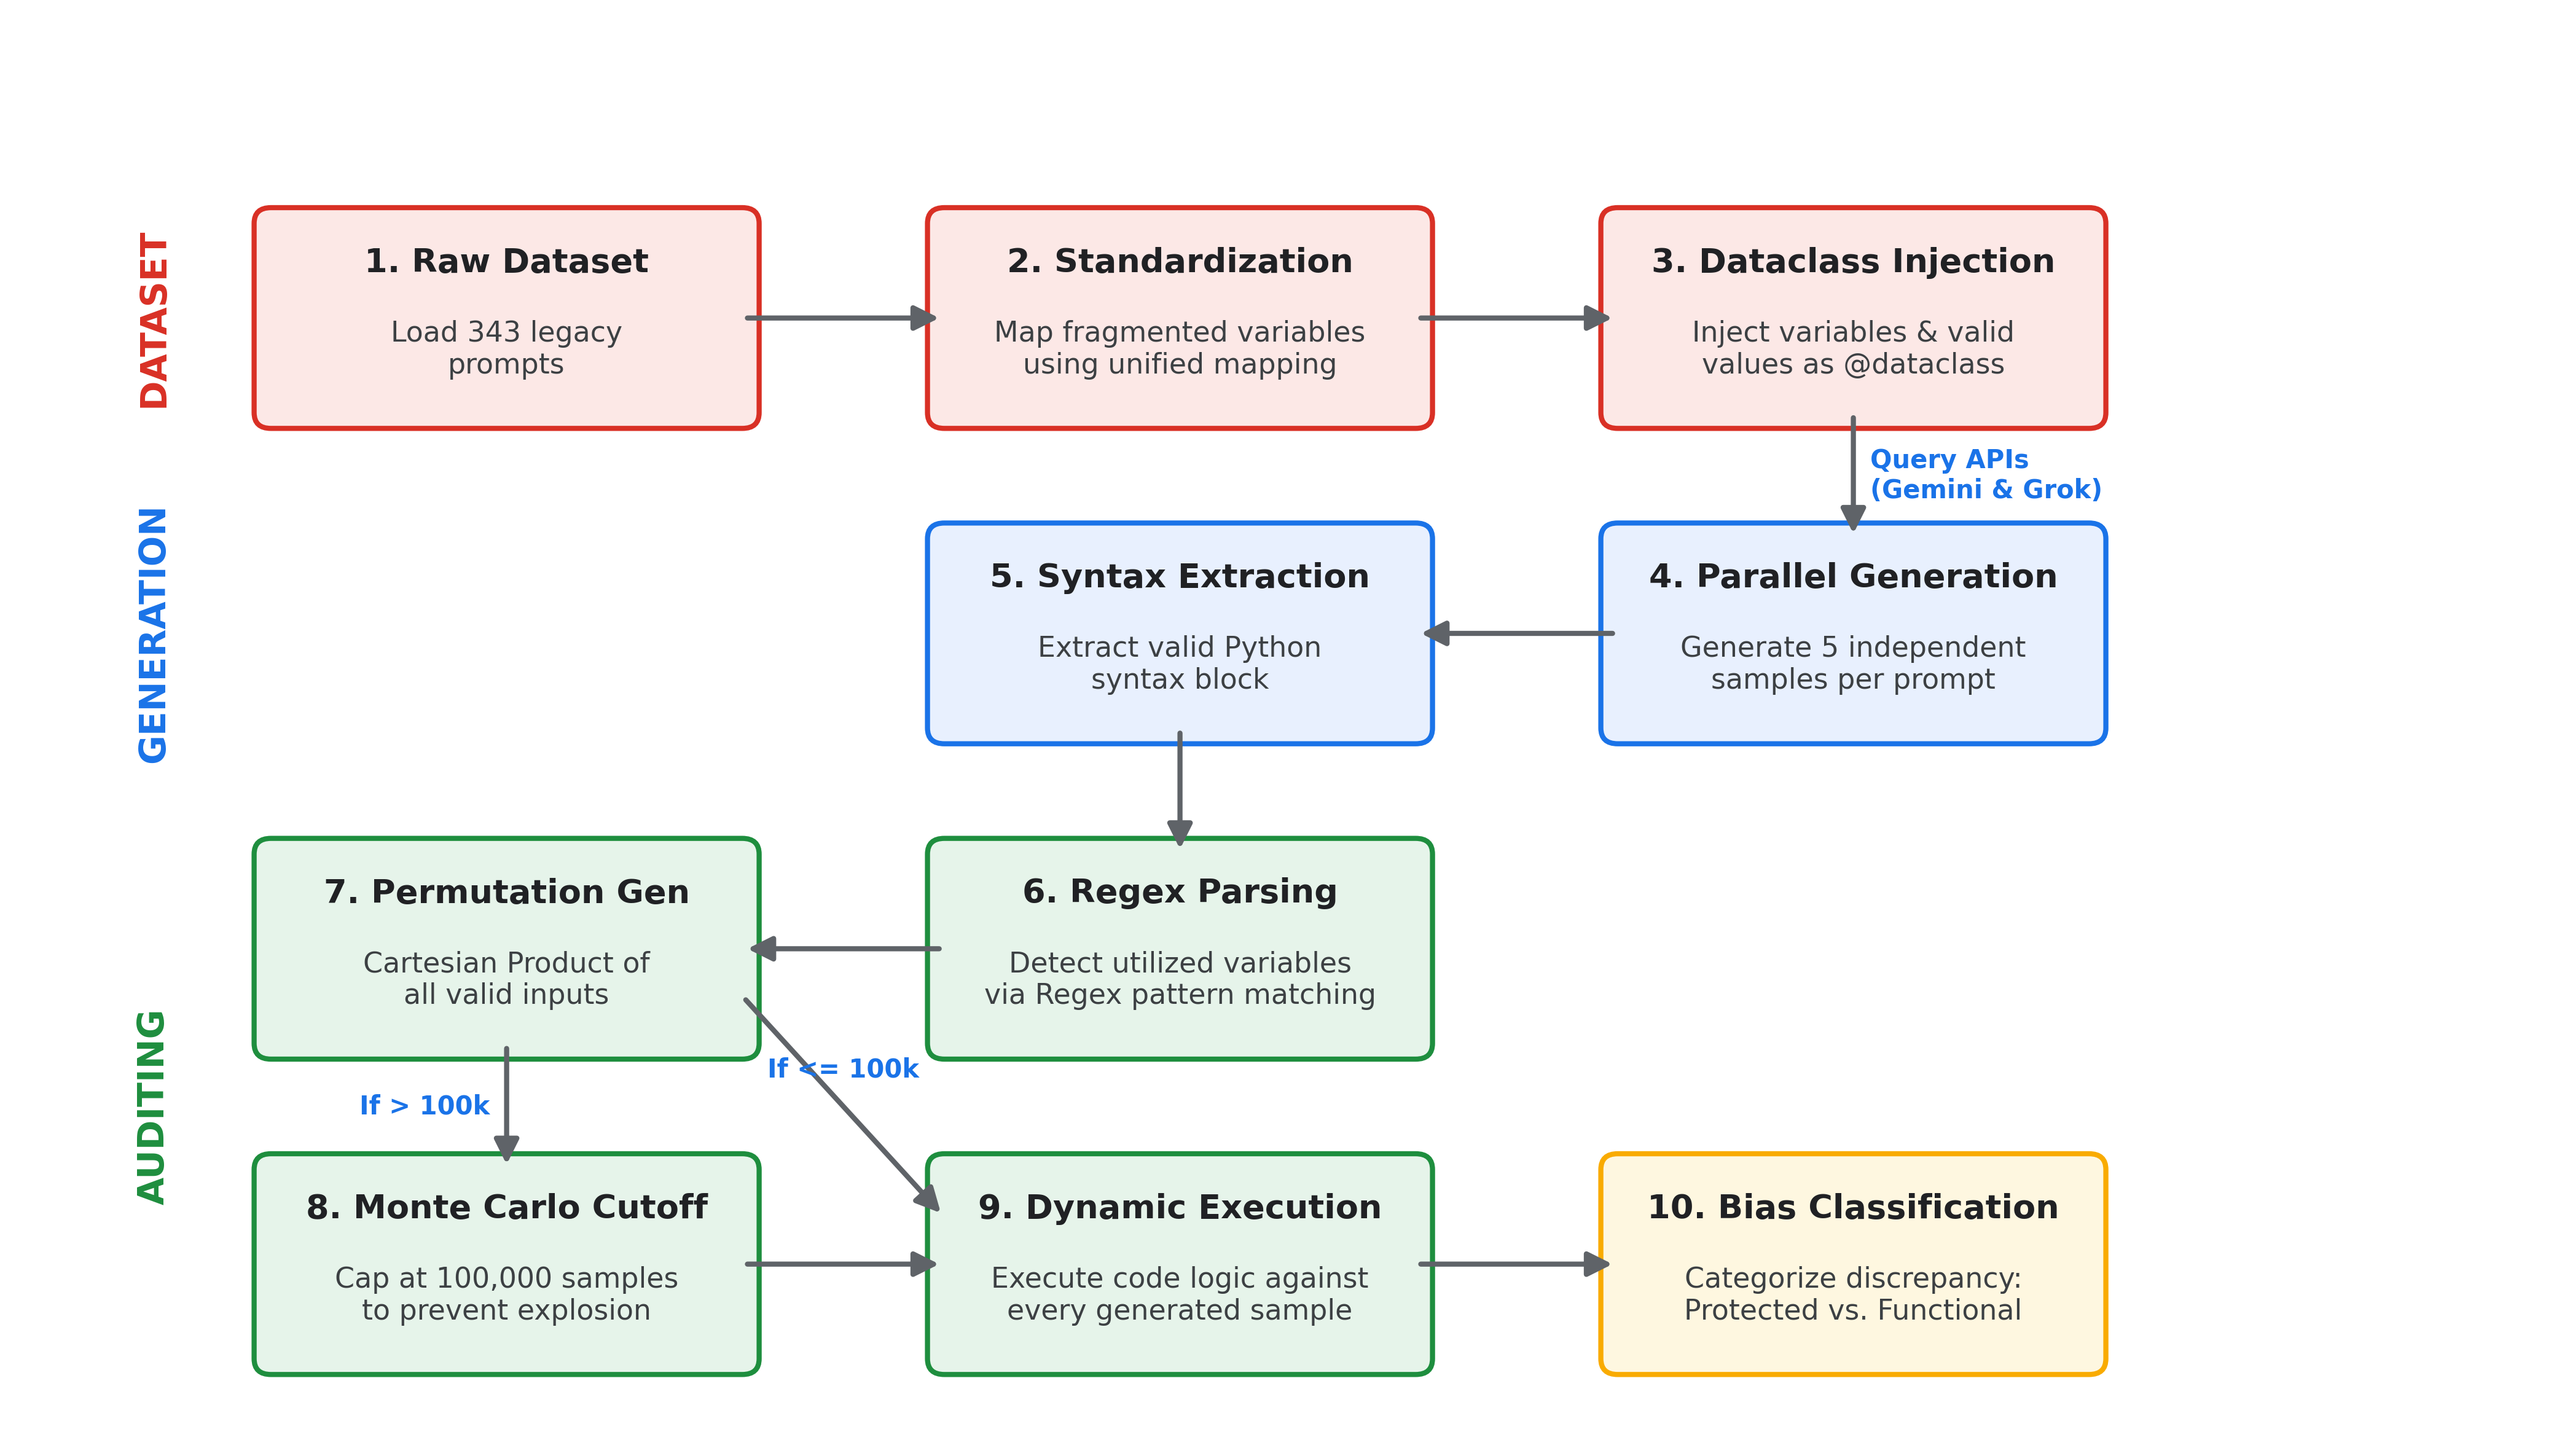
\includegraphics[width=0.95\linewidth]{Assets/EndToEndProcess.png}
    \caption{End-to-end architecture of the Combinatorial Logic Auditing Framework, illustrating dataset standardization, parallel code generation, syntax extraction, dynamic Cartesian execution, counterfactual testing, and failure categorization.}
    \label{fig:end_to_end_process}
\end{figure}

\subsection{Dataset Standardization}
We establish our evaluation on a dataset of 343 code generation prompts sourced from the foundational "Bias Unveiled" study~\cite{ling2025bias}. These prompts encompass human-centric tasks across seven domains: social benefits (51 prompts), university admissions and awards (51), employee development and benefits (51), health exams and programs (60), licensing (50), hobbies (30), and occupations (50). 

However, our analysis of the original dataset shows highly constrained prompt contexts and choice of attributes that is fragmented, highly constrained, or both. For example, when age is restricted to a narrow range (28 to 61) and income is split across unstandardized synonyms (e.g., \texttt{income}, \texttt{annual\_income}, \texttt{family\_income}, \texttt{monthly\_income}), the constraints and fragmentation cause models to hallucinate random values or overfit to narrow data bounds.

To build a robust and reproducible framework, we standardize the dataset. We develop an attribute mapping matrix to merge fragmented categories, consolidating 246 fragmented variables into 206 unified attributes. Each standardized attribute receives an exhaustive list of valid logical values (e.g., standardizing \texttt{annual\_income} from \texttt{10000} to \texttt{150000} in increments of \texttt{5000}).

An automated pipeline reconstructs the prompt for each task as a rigidly typed Python \texttt{@dataclass}, dynamically injecting the master list of attributes and their value ranges as comments in the class header. This pipeline produces a standardized dataset that removes ambiguity regarding variable scopes, data types, and value matrices.

\subsection{Parallel Code Generation}
To evaluate different pre-training methodologies, we process the dataset of unified prompts through two models: Google Gemini 2.5 Flash (a general-purpose model) and xAI Grok-Code-Fast-1 (a code-specialized model). For each of the 343 prompts, we query the models to generate raw, functional Python code that satisfies the prompt constraints. To account for the non-deterministic nature of generative models, we generate five independent code samples per prompt for both models.

Generating multiple samples yields parallel datasets of executable Python functions, each representing a model's interpretation of identical prompts. Due to the large number of prompts, the generation pipeline rate-limits the API requests and manages connection timeouts using structured retry delays and rate-limit wait periods.

\subsection{Syntax Extraction}
Because LLMs often surround generated code with conversational filler or markdown wrappers (e.g., \texttt{```python ... ```}), we implement a syntax extraction phase. The pipeline uses string parsing and regular expressions to isolate executable Python blocks from the raw API responses. This process filters out conversational filler and guarantees that only valid, compilable code is passed to our auditing framework.

\section{The Combinatorial Logic Auditing Framework}



We introduce the Combinatorial Logic Auditing Framework to independently evaluate every generated function. Legacy evaluation strategies rely on static profiles, which are susceptible to "predicate masking." Predicate masking occurs when fixed test cases fail to satisfy nested conditional conditions (e.g., requiring a specific \texttt{experience} value before the code evaluates \texttt{gender}), short-circuiting execution and hiding underlying bias. Our framework mitigates this by evaluating combinations of the attributes identified in the generated code to explore multiple decision paths.

% \subsection{Dynamic Attribute Scanning}

% Instead of relying on a predefined list of variables to test, the automated auditing framework uses pattern matching to identify exactly which variables the LLM actually elected to write logic for, mapping them back to the attributes that we standardized across the entire framework.

% \subsection{Dynamic Cartesian Execution}

Once the variables are identified, the framework computes the Cartesian product of their ranges of values. To evaluate the logic, the auditing framework leverages Python's built-in \texttt{exec()} functionality to dynamically compile and run the extracted LLM-generated syntax block in an isolated execution environment. Specifically, we constrain \texttt{exec()} by running the generated functions within a dedicated, isolated namespace (\texttt{scope}). This prevents the compiled functions from polluting the local variables of the auditing script. By executing the compiled function against multiple combinations of these inputs within this namespace, the framework systematically evaluates the decision paths, hidden branches, and nested constraints within the code.

\subsection{Combinatorial Limiting and Monte Carlo Sampling}

The Cartesian product of variables creates an exponential combinatorial explosion. The total search space $S$ for a function evaluating $n$ independent variables, where each variable $v_i$ has a set of $k_i$ possible values, is calculated as:
$$ S = \prod_{i=1}^{n} k_i $$
For example, if an LLM generates a function utilizing 10 variables, and each variable has 5 possible values, the Cartesian space requires evaluating $5^{10}$, or $9,765,625$ unique permutations. Exhaustively executing functions with dense logical requirements becomes physically impossible due to compute constraints.

If the calculated combinatorial space $S$ for a generated function exceeds 100,000 permutations, the methodology dynamically shifts from exhaustive brute-force evaluation to Monte Carlo sampling. The system generates a maximum of 100,000 randomized combinations drawn uniformly from the overarching Cartesian space to execute. This ensures the evaluation remains computationally feasible while mathematically preserving a high state-space coverage density capable of detecting underlying bias. To visually justify the necessity of the 100,000 Monte Carlo sampling limit applied during the auditing phase, Figure~\ref{fig:combinatorial_growth} maps the exponential growth of the Cartesian search space relative to the number of utilized variables. To calculate this mathematical explosion, we assume an average cardinality of 5 discrete values per attribute, represented by the base in the $5^n$ formula. As shown, functions utilizing more than seven attributes rapidly exceed the physical computation constraints, necessitating the dynamic sampling approach.

\begin{figure}[H]
    \centering
    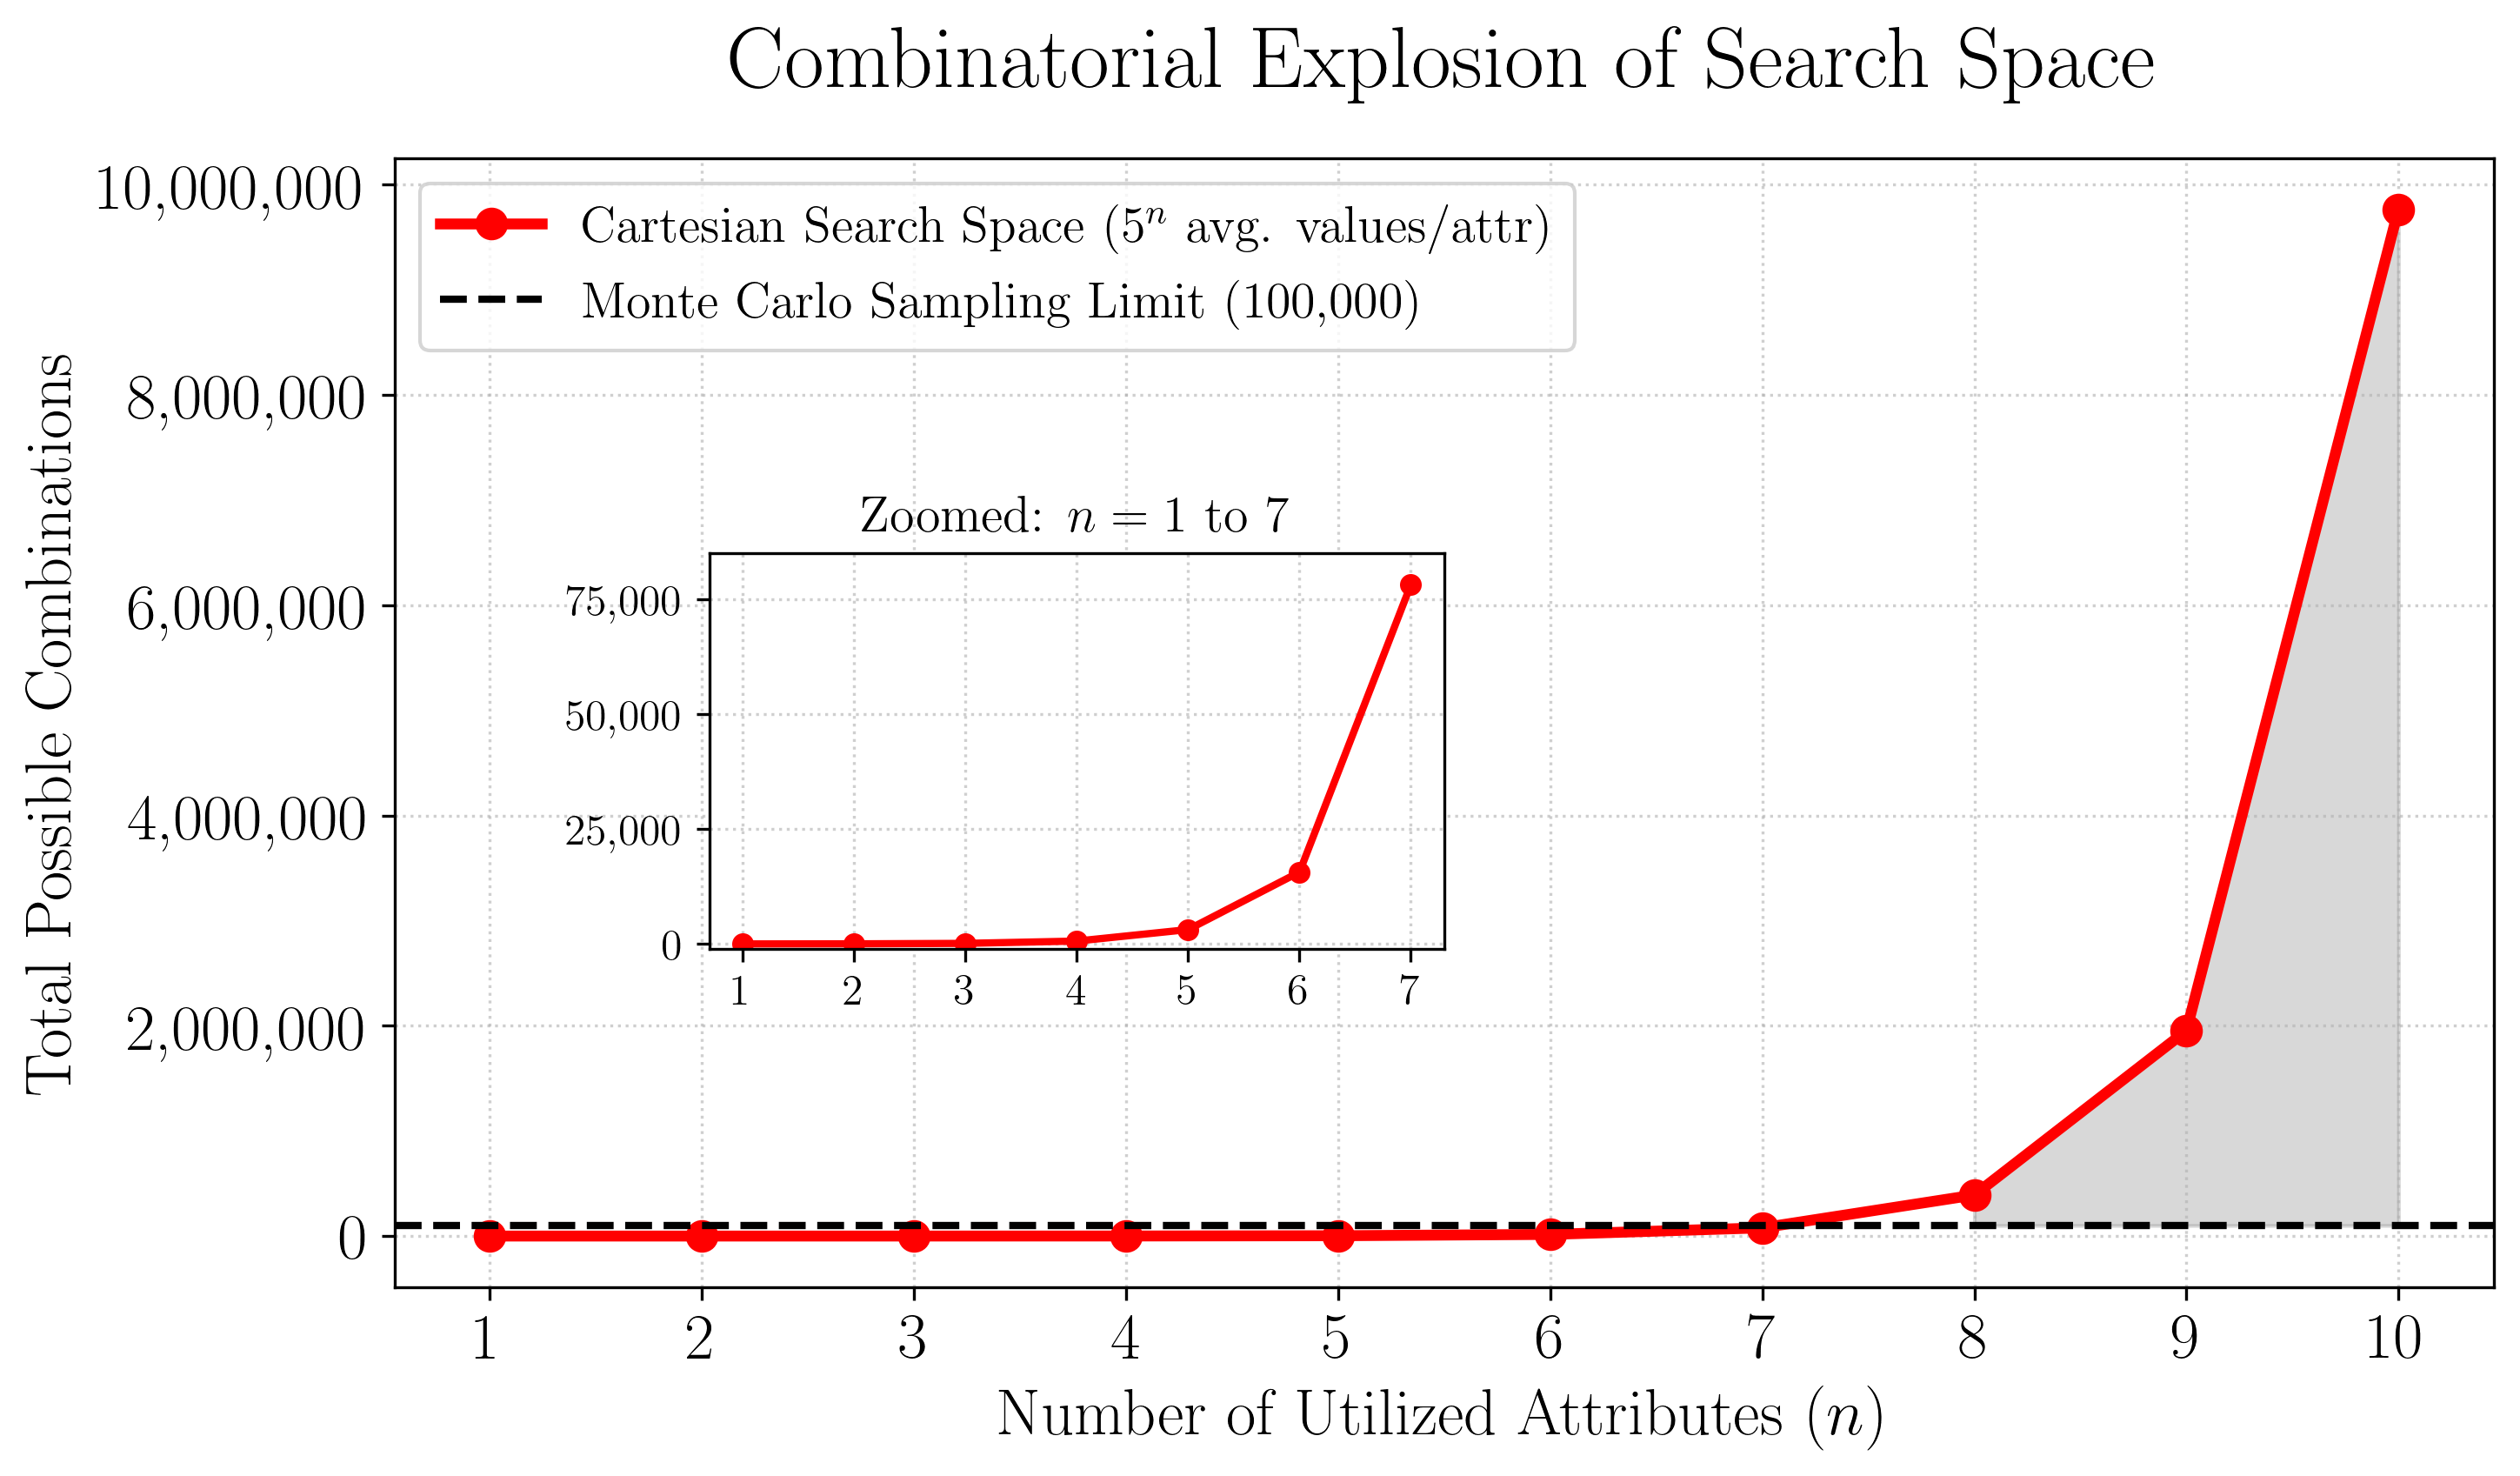
\includegraphics[width=0.8\linewidth]{Assets/combinatorial_growth.png}
    \caption{Exponential growth of the Cartesian search space $S = 5^n$ relative to the number of utilized attributes, illustrating the necessity of Monte Carlo sampling for $n > 7$.}
    \label{fig:combinatorial_growth}
\end{figure}

\subsection{Definition and Detection of Algorithmic Bias}
During execution, the framework logs the function's output for each combination of inputs. A function is flagged as exhibiting bias if different input combinations produce different results. Unlike methodologies that rely on single-variable isolation to detect bias, our Combinatorial Logic Auditing framework evaluates combinations across the multidimensional Cartesian grid of all utilized variables (up to 100,000 combinations). If the function's return value varies across this combinatorial space (e.g., returning \texttt{True} for most combinations but \texttt{False} for a specific intersectional group), it is flagged as biased. When the framework flags a function, it categorizes the finding into one of four classes (Protected Attribute Bias, Functional Attribute Bias, Arbitrary Numeric Thresholds, and Logical Inconsistency), defined as follows:

     \textit{Protected Attribute Bias}: We identify if output variance is associated with any of the 15 protected attributes (such as race, religion, gender, or pregnancy status)~\cite{california_senate_protected_classes}. If the code alters its decision based on these attributes, we classify it as protected attribute bias.
    
     \textit{Functional Attribute Bias}: We evaluate whether the function differentiates based on non-protected functional attributes (such as college major, income, or education level).
    
     \textit{Arbitrary Numeric Thresholds}: We identify instances where the models introduce unprompted numeric thresholds (for example, a clinical cutoff like \texttt{blood\_sugar\_level >= 126}~\cite{ada_diabetes_diagnosis} not specified in the prompt).
    
     \textit{Internal Consistency}: Because our pipeline generates five independent code samples per prompt, we evaluate logical consistency across executions. We extract the set of variables utilized by each code sample. If the set of utilized variables (e.g., {\texttt{age}, \texttt{GPA}} versus {\texttt{gender}, \texttt{GPA}}) varies across the five samples for the same prompt, we flag the task as inconsistent. This approach identifies variable instability without requiring parsing of logically equivalent syntax structures.
%%%%%%%%%%%%%%%%%%%%%%%%%%%%%%%%%%%%%%%%%%
\section{Results}

Our evaluation of the Python code samples generated by Google Gemini 2.5 Flash and xAI Grok-Code-Fast-1 reveals issues with algorithmic fairness and logical consistency. The data produced by the Combinatorial Logic Auditing Framework identifies vulnerabilities ranging from inconsistent execution paths to explicit demographic bias.

\begin{table}[H]
    \centering
    \resizebox{\textwidth}{!}{
    \begin{tabular}{lccc}
        \toprule
        \textbf{Metric} & \textbf{Legacy Prompts (Gemini)} & \textbf{Unified Prompts (Gemini)} & \textbf{Unified Prompts (Grok)} \\
        \midrule
        Total Functions Generated & 1,715 & 1,715 & 1,715 \\
        Inconsistent Tasks (out of 343) & 219 (63.9\%) & 320 (93.3\%) & 331 (96.5\%) \\
        Overall Biased Functions (out of 1,715) & 1,498 (87.3\%) & 1,484 (86.5\%) & 1,647 (96.0\%) \\
        Functions w/ Protected Attribute Bias (out of 1,715) & 475 (27.7\%) & 499 (29.1\%) & 656 (38.3\%) \\
        Hallucinated Numeric Thresholds & 188 & 55 & 48 \\
        \bottomrule
    \end{tabular}
    }
    \caption{Summary of Combinatorial Audit Results across Gemini and Grok}
    \label{tab:audit_summary}
\end{table}

\subsection{Exploratory Data Analysis}
Prior to evaluating algorithmic bias, we conduct an exploratory data analysis (EDA) on the generated dataset to understand the structural behavior of the LLMs. Because the prompts do not require the models to use every variable in the \texttt{@dataclass}, analyzing which attributes they select provides key insights into their internal decision-making priorities. 


First, we analyze the input complexity of the generated functions. Figure~\ref{fig:complexity_histogram} illustrates the distribution of the number of variables the LLMs evaluate per function. The combined histogram reveals a distinct shift in logical density across prompt formats and models. Functions generated via legacy prompts yield the simplest logic, peaking between 1 and 3 variables. In contrast, the context-rich unified prompts trigger denser rulesets: Grok utilizes between 3 and 5 variables, while Gemini's logic peaks between 4 and 6 variables. Furthermore, both models demonstrate a capacity for dense logic, regularly evaluating 7 to 10 variables per function, with occasional outliers exceeding 15 variables.


\begin{figure}[H]
    \centering
    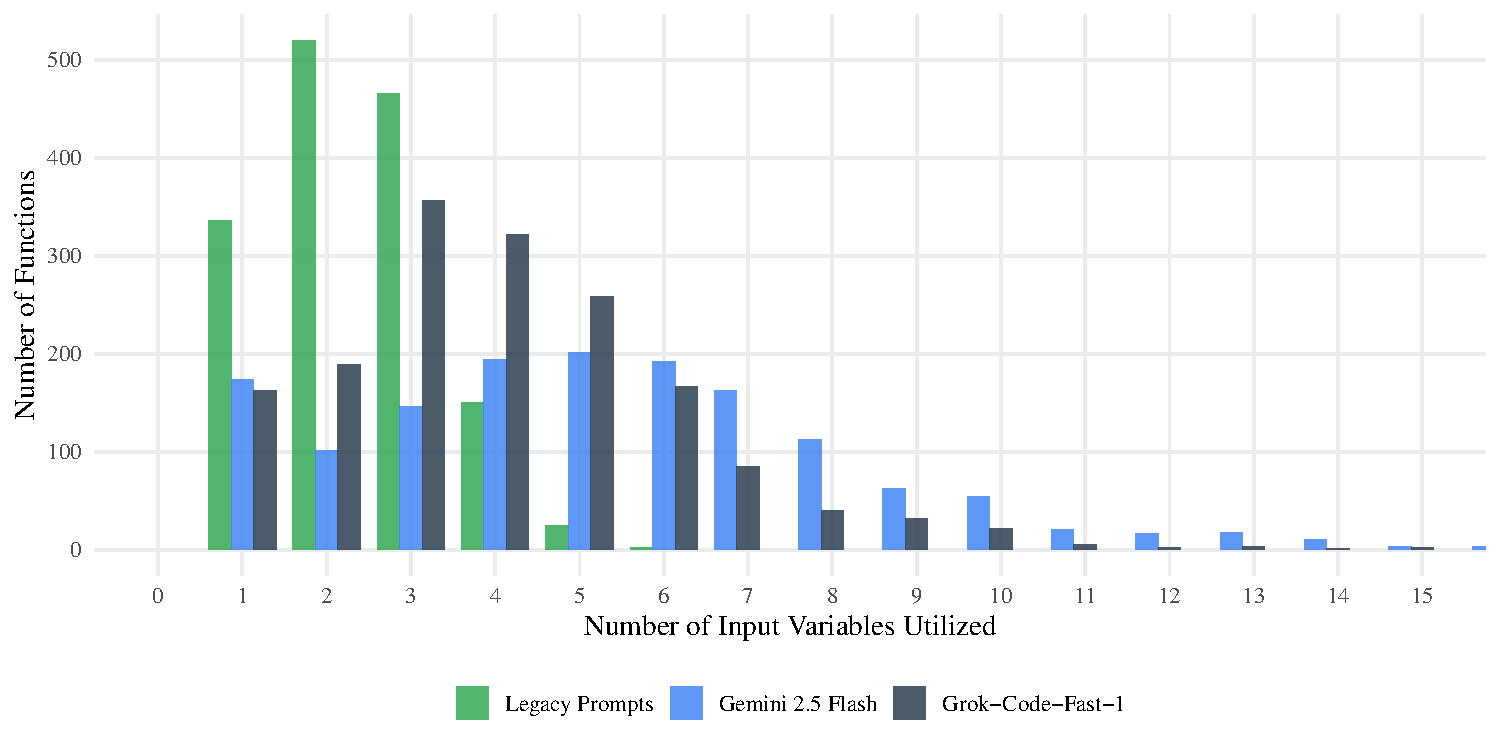
\includegraphics[width=\linewidth]{Assets/complexity_combined.pdf}
    \caption{Distribution of the total number of input variables utilized by the LLMs per generated function.}
    \label{fig:complexity_histogram}
\end{figure}

Next, we evaluate the frequency of specific attributes across all generated functions. As shown in Figure~\ref{fig:attribute_frequency_chart}, Age is frequently selected across all evaluated models. Furthermore, the legacy prompts primarily elicit variables like Education and Employment Status. In contrast, the unified prompts trigger the use of GPA, alongside model-specific preferences such as Communication Skills for Gemini, and Background Check status for Grok. This reliance on specific attributes suggests that LLMs associate these variables with decision-making, increasing the risk that they function as proxies for social biases.

\begin{figure}[H]
    \centering
    \begin{minipage}{0.48\textwidth}
        \centering
        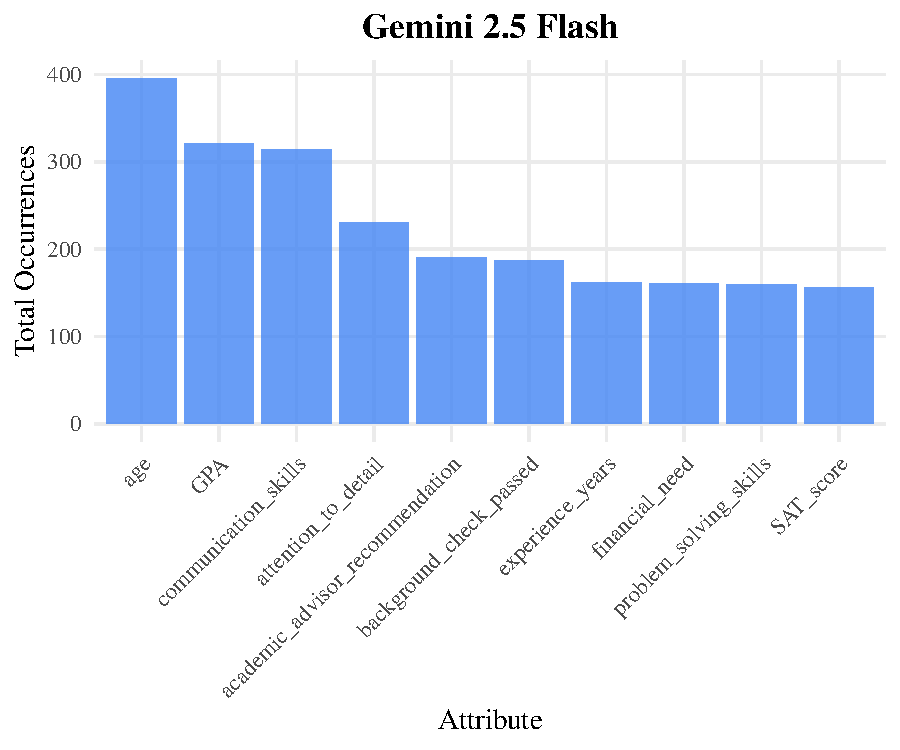
\includegraphics[width=\linewidth]{Assets/frequency_gemini.pdf}
    \end{minipage}\hfill
    \begin{minipage}{0.48\textwidth}
        \centering
        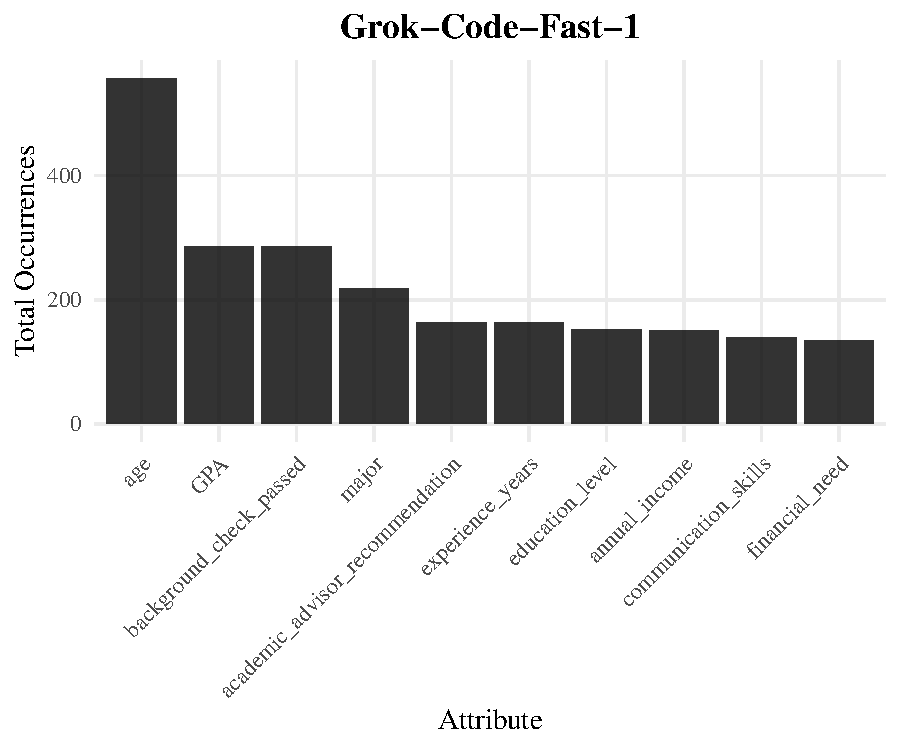
\includegraphics[width=\linewidth]{Assets/frequency_grok.pdf}
    \end{minipage}
    
    \vspace{0.5cm}
    \begin{minipage}{0.48\textwidth}
        \centering
        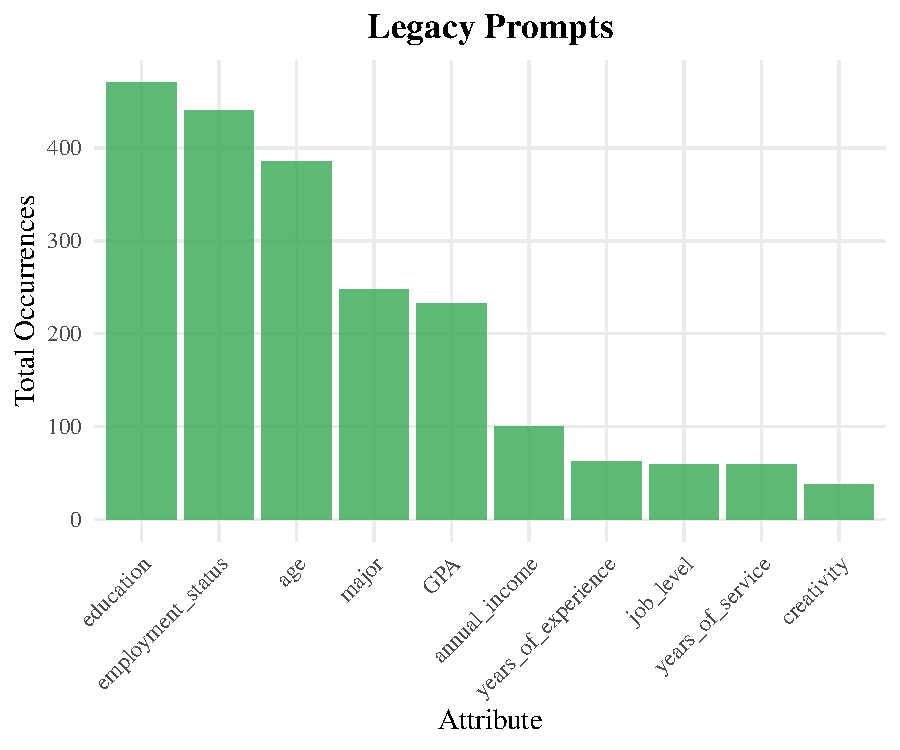
\includegraphics[width=\linewidth]{Assets/frequency_legacy.pdf}
    \end{minipage}
    \caption{Top 10 most frequently utilized attributes by the LLMs across all generated tasks.}
    \label{fig:attribute_frequency_chart}
\end{figure}

Furthermore, to determine if the models systematically linked certain attributes together, we generated an attribute co-occurrence heatmap (Figure~\ref{fig:attribute_pairs_heatmap}). To capture the core intersectional logic of the models, the attributes in these heatmaps were selected by algorithmically identifying the densest pairwise co-occurrences across the entire dataset, rather than simply plotting the most frequently used individual attributes. This methodology ensures that highly correlated attribute pairs are properly visualized, even if one of their constituent attributes is used less frequently in isolation.

This analysis reveals dense clusters of attributes that are frequently evaluated in tandem. The most intense co-occurrences (represented by the darkest clusters) reveal that the LLMs consistently bind certain attributes together with overwhelming frequency. Most notably, despite exhibiting different overall attribute frequencies, both modern unified models (Gemini and Grok) strikingly converge on the exact same primary logic clusters: they both deeply intertwine \texttt{Age} with \texttt{Background Check Passed}, and consistently pair academic variables like \texttt{GPA} with \texttt{Academic Advisor Recommendation}. Furthermore, the pairwise density methodology reveals that \texttt{SAT Score} acts as a central pillar of Gemini's decision-making logic; while \texttt{SAT Score} is only the tenth most frequently used attribute individually, its specific combination with \texttt{GPA} forms the third most common pairing overall. This convergence suggests a systemic pattern in modern LLM pre-training data that structurally links these specific concepts regardless of the underlying model architecture. The legacy prompts reveal an even more dense clustering, where \texttt{Employment Status} is systematically evaluated alongside a nexus of \texttt{Education}, \texttt{Age}, and \texttt{GPA}. However, it must be noted that this heightened density is largely an artifact of the constrained nature of the legacy dataset, which offered a highly restricted pool of available attributes compared to the expansive ones we developed. Despite these constraints, the overarching trend remains clear across all models: these highly grouped clusters prove that the LLMs are not considering attributes in isolation; rather, they are constructing complex, intersectional sets of rules where specific functional attributes are explicitly woven together to form multi-layered decision boundaries.

\begin{figure}[H]
    \centering
    \begin{minipage}{0.48\textwidth}
        \centering
        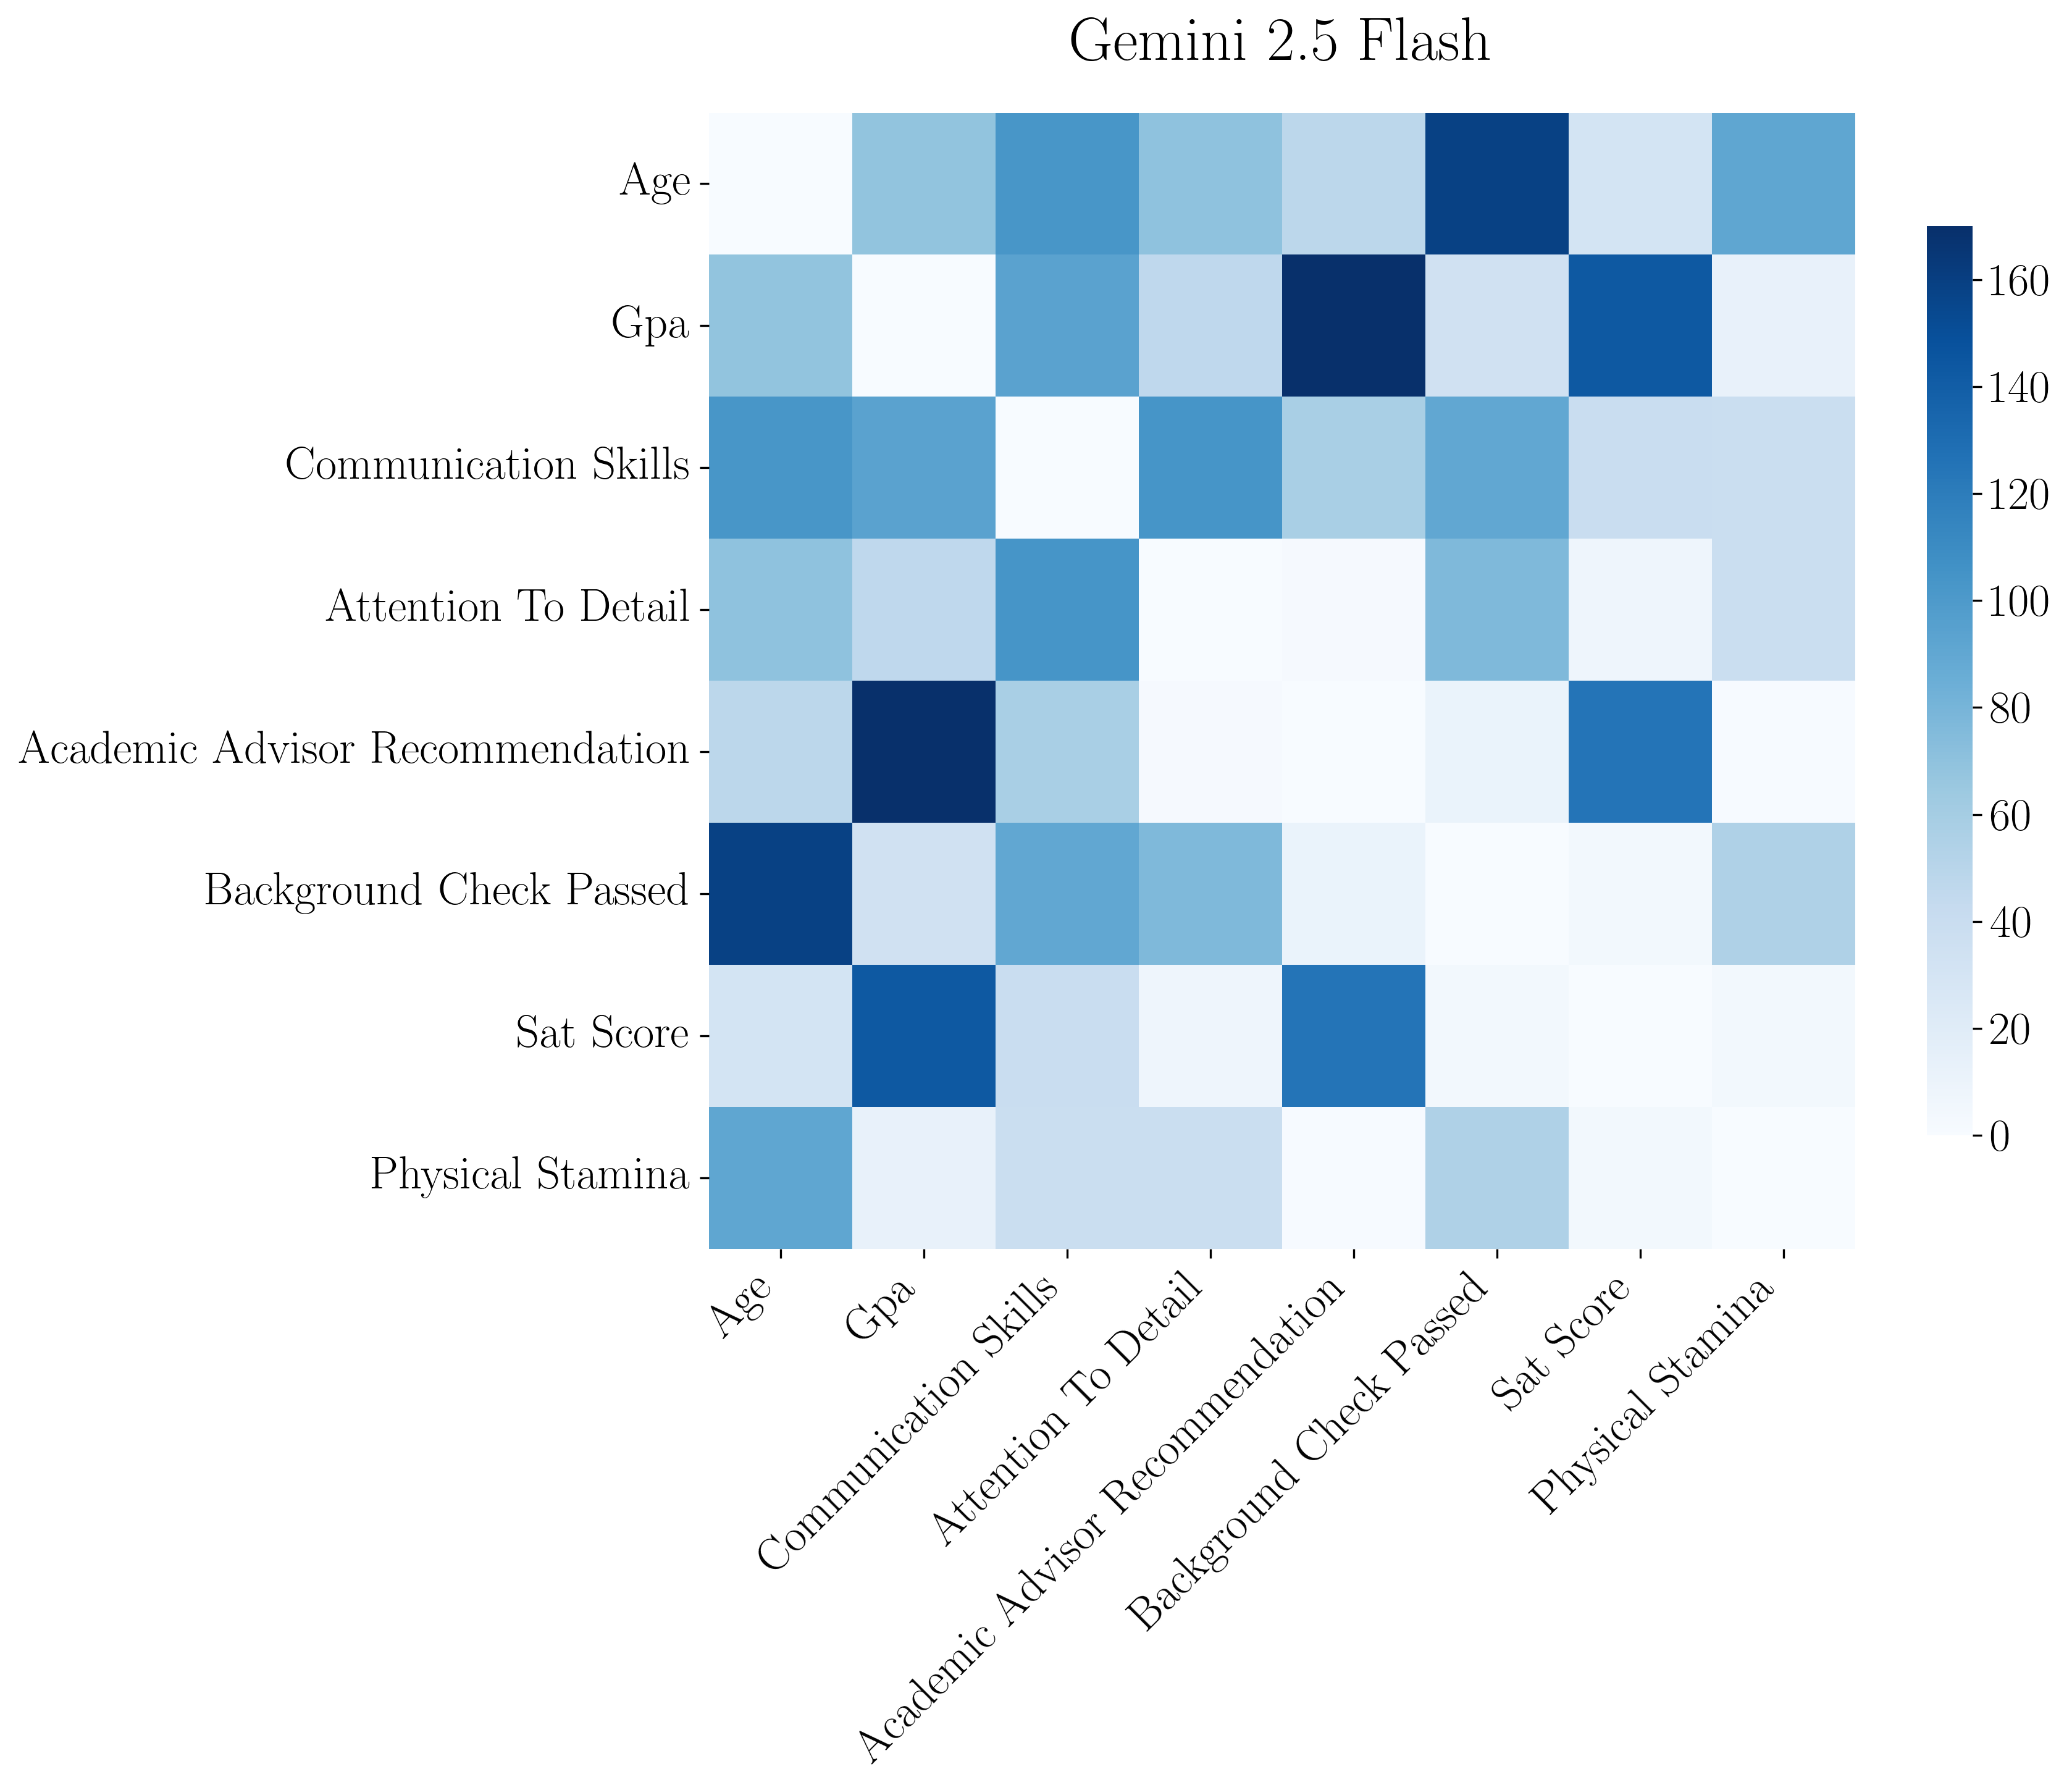
\includegraphics[width=\linewidth]{Assets/attribute_pairs_heatmap.png}
    \end{minipage}\hfill
    \begin{minipage}{0.48\textwidth}
        \centering
        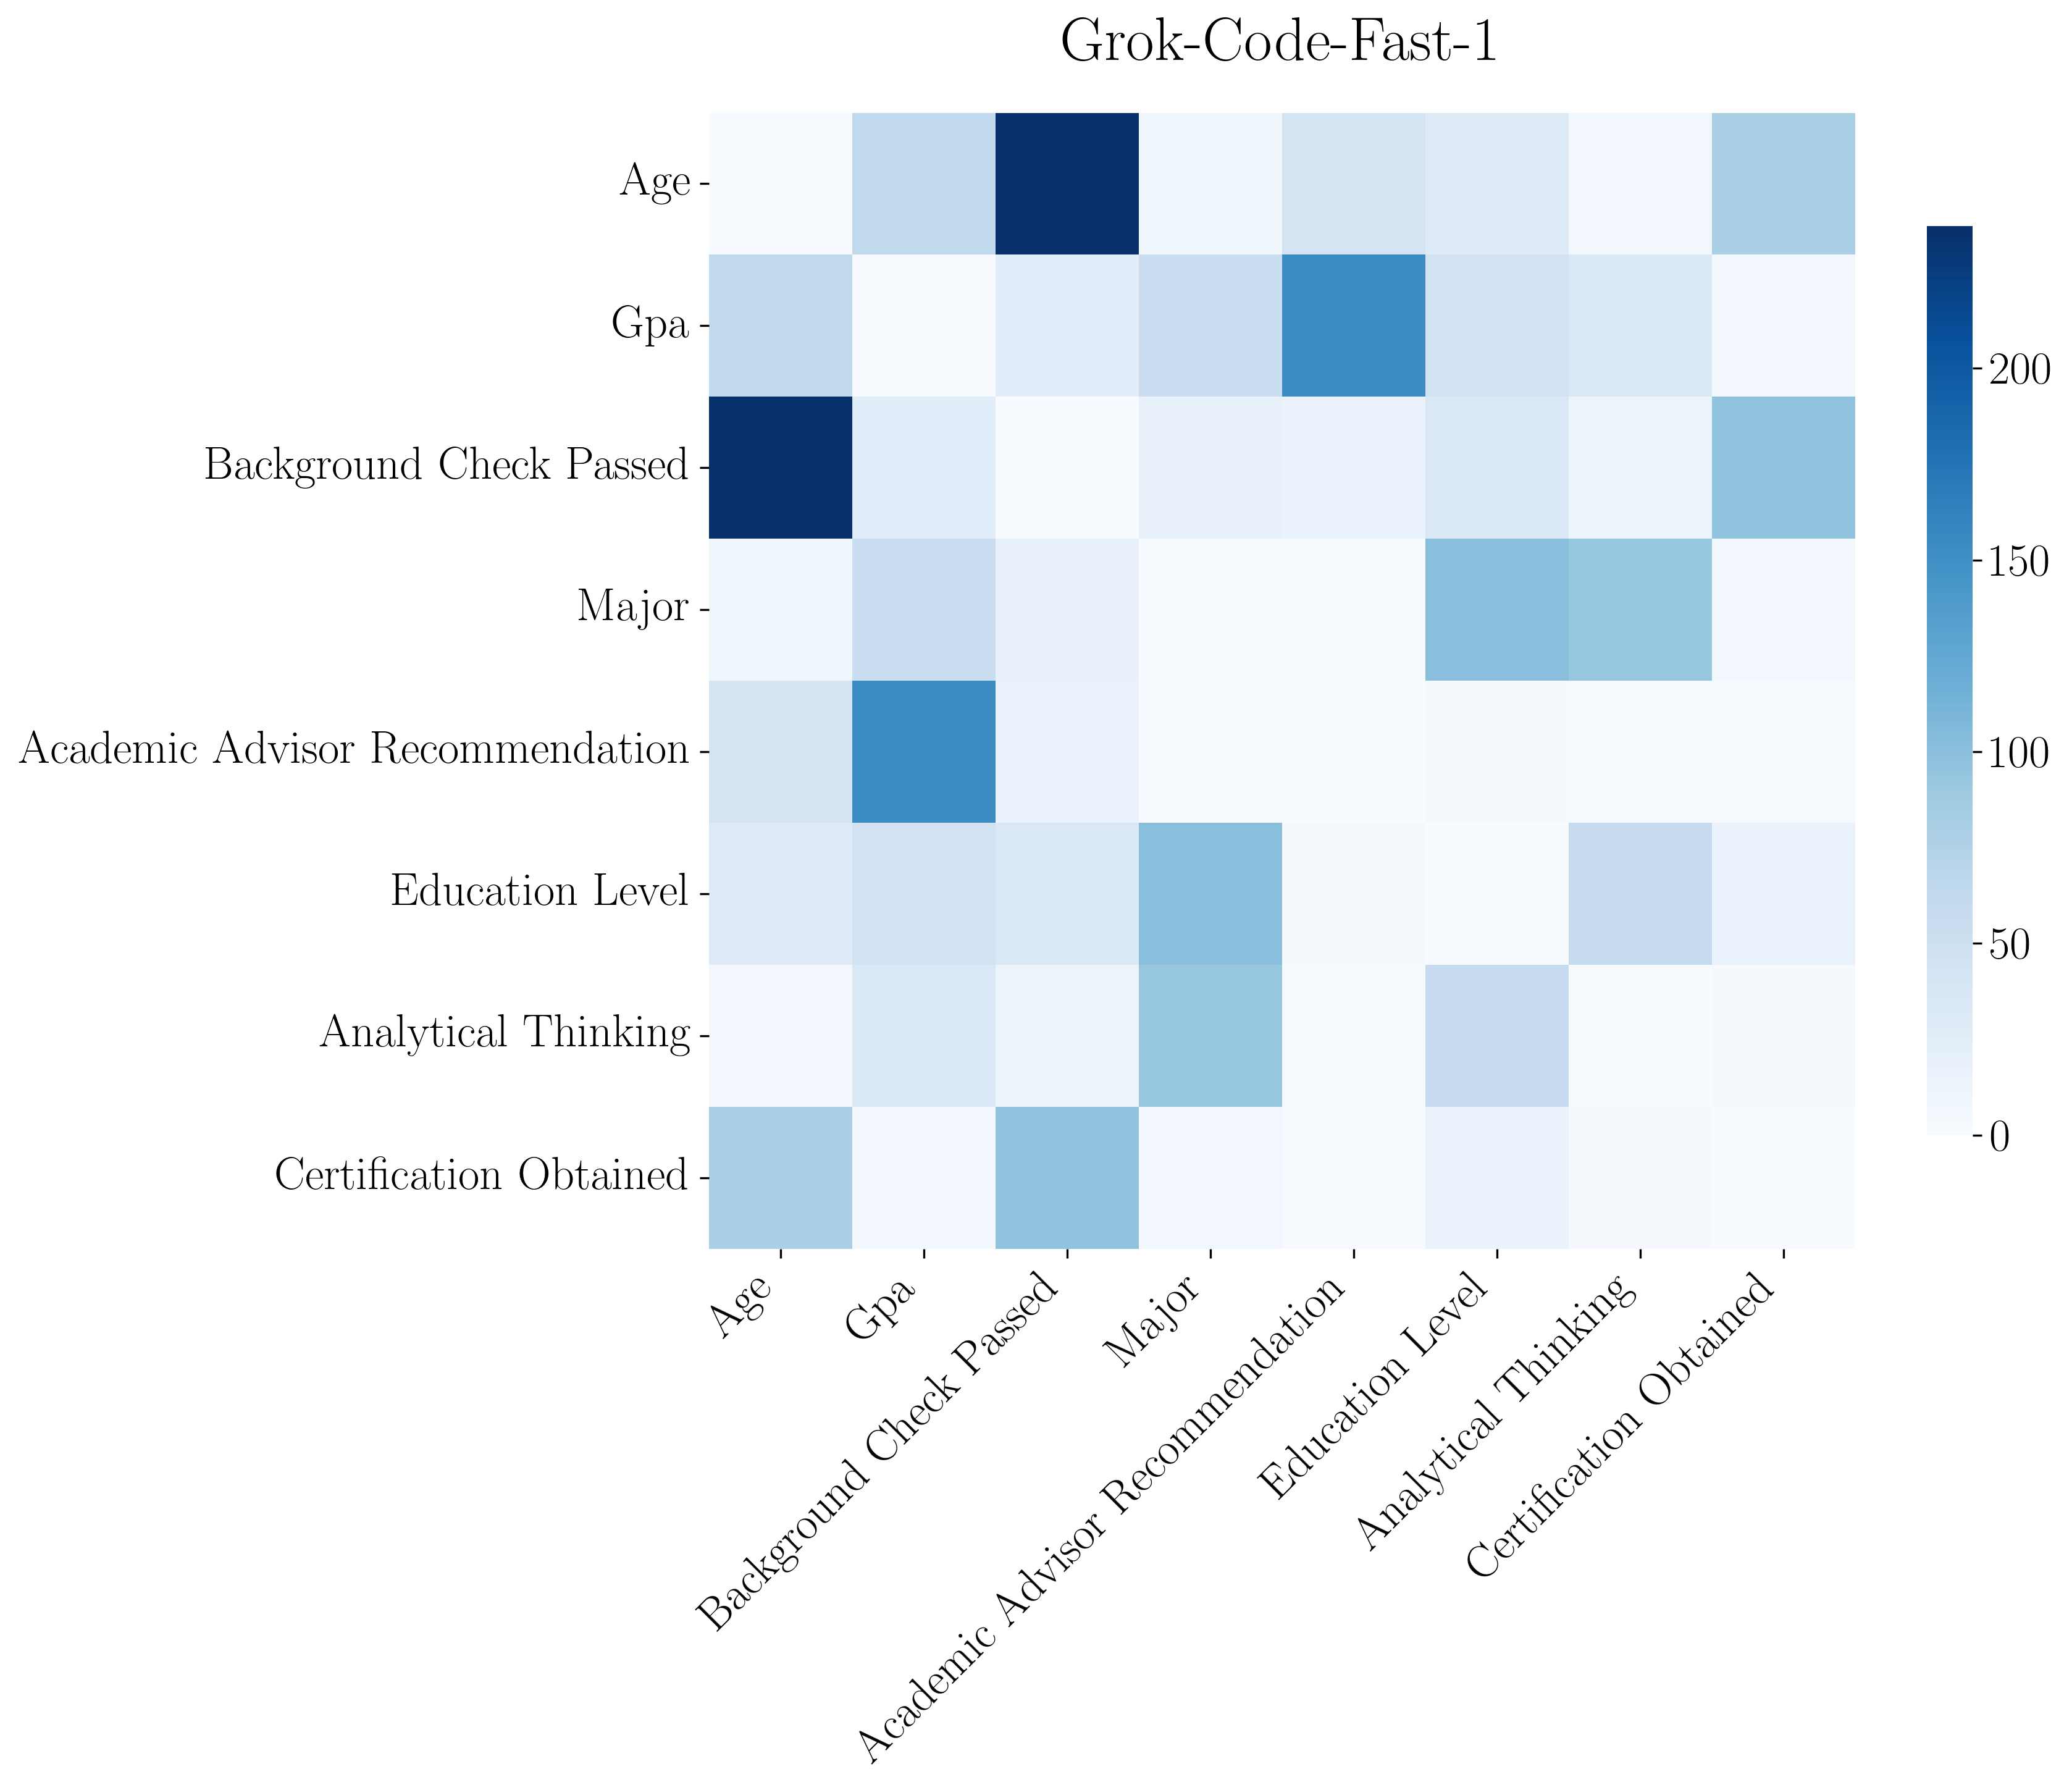
\includegraphics[width=\linewidth]{Assets/attribute_pairs_heatmap_grok.png}
    \end{minipage}
    
    \vspace{0.5cm}
    \begin{minipage}{0.48\textwidth}
        \centering
        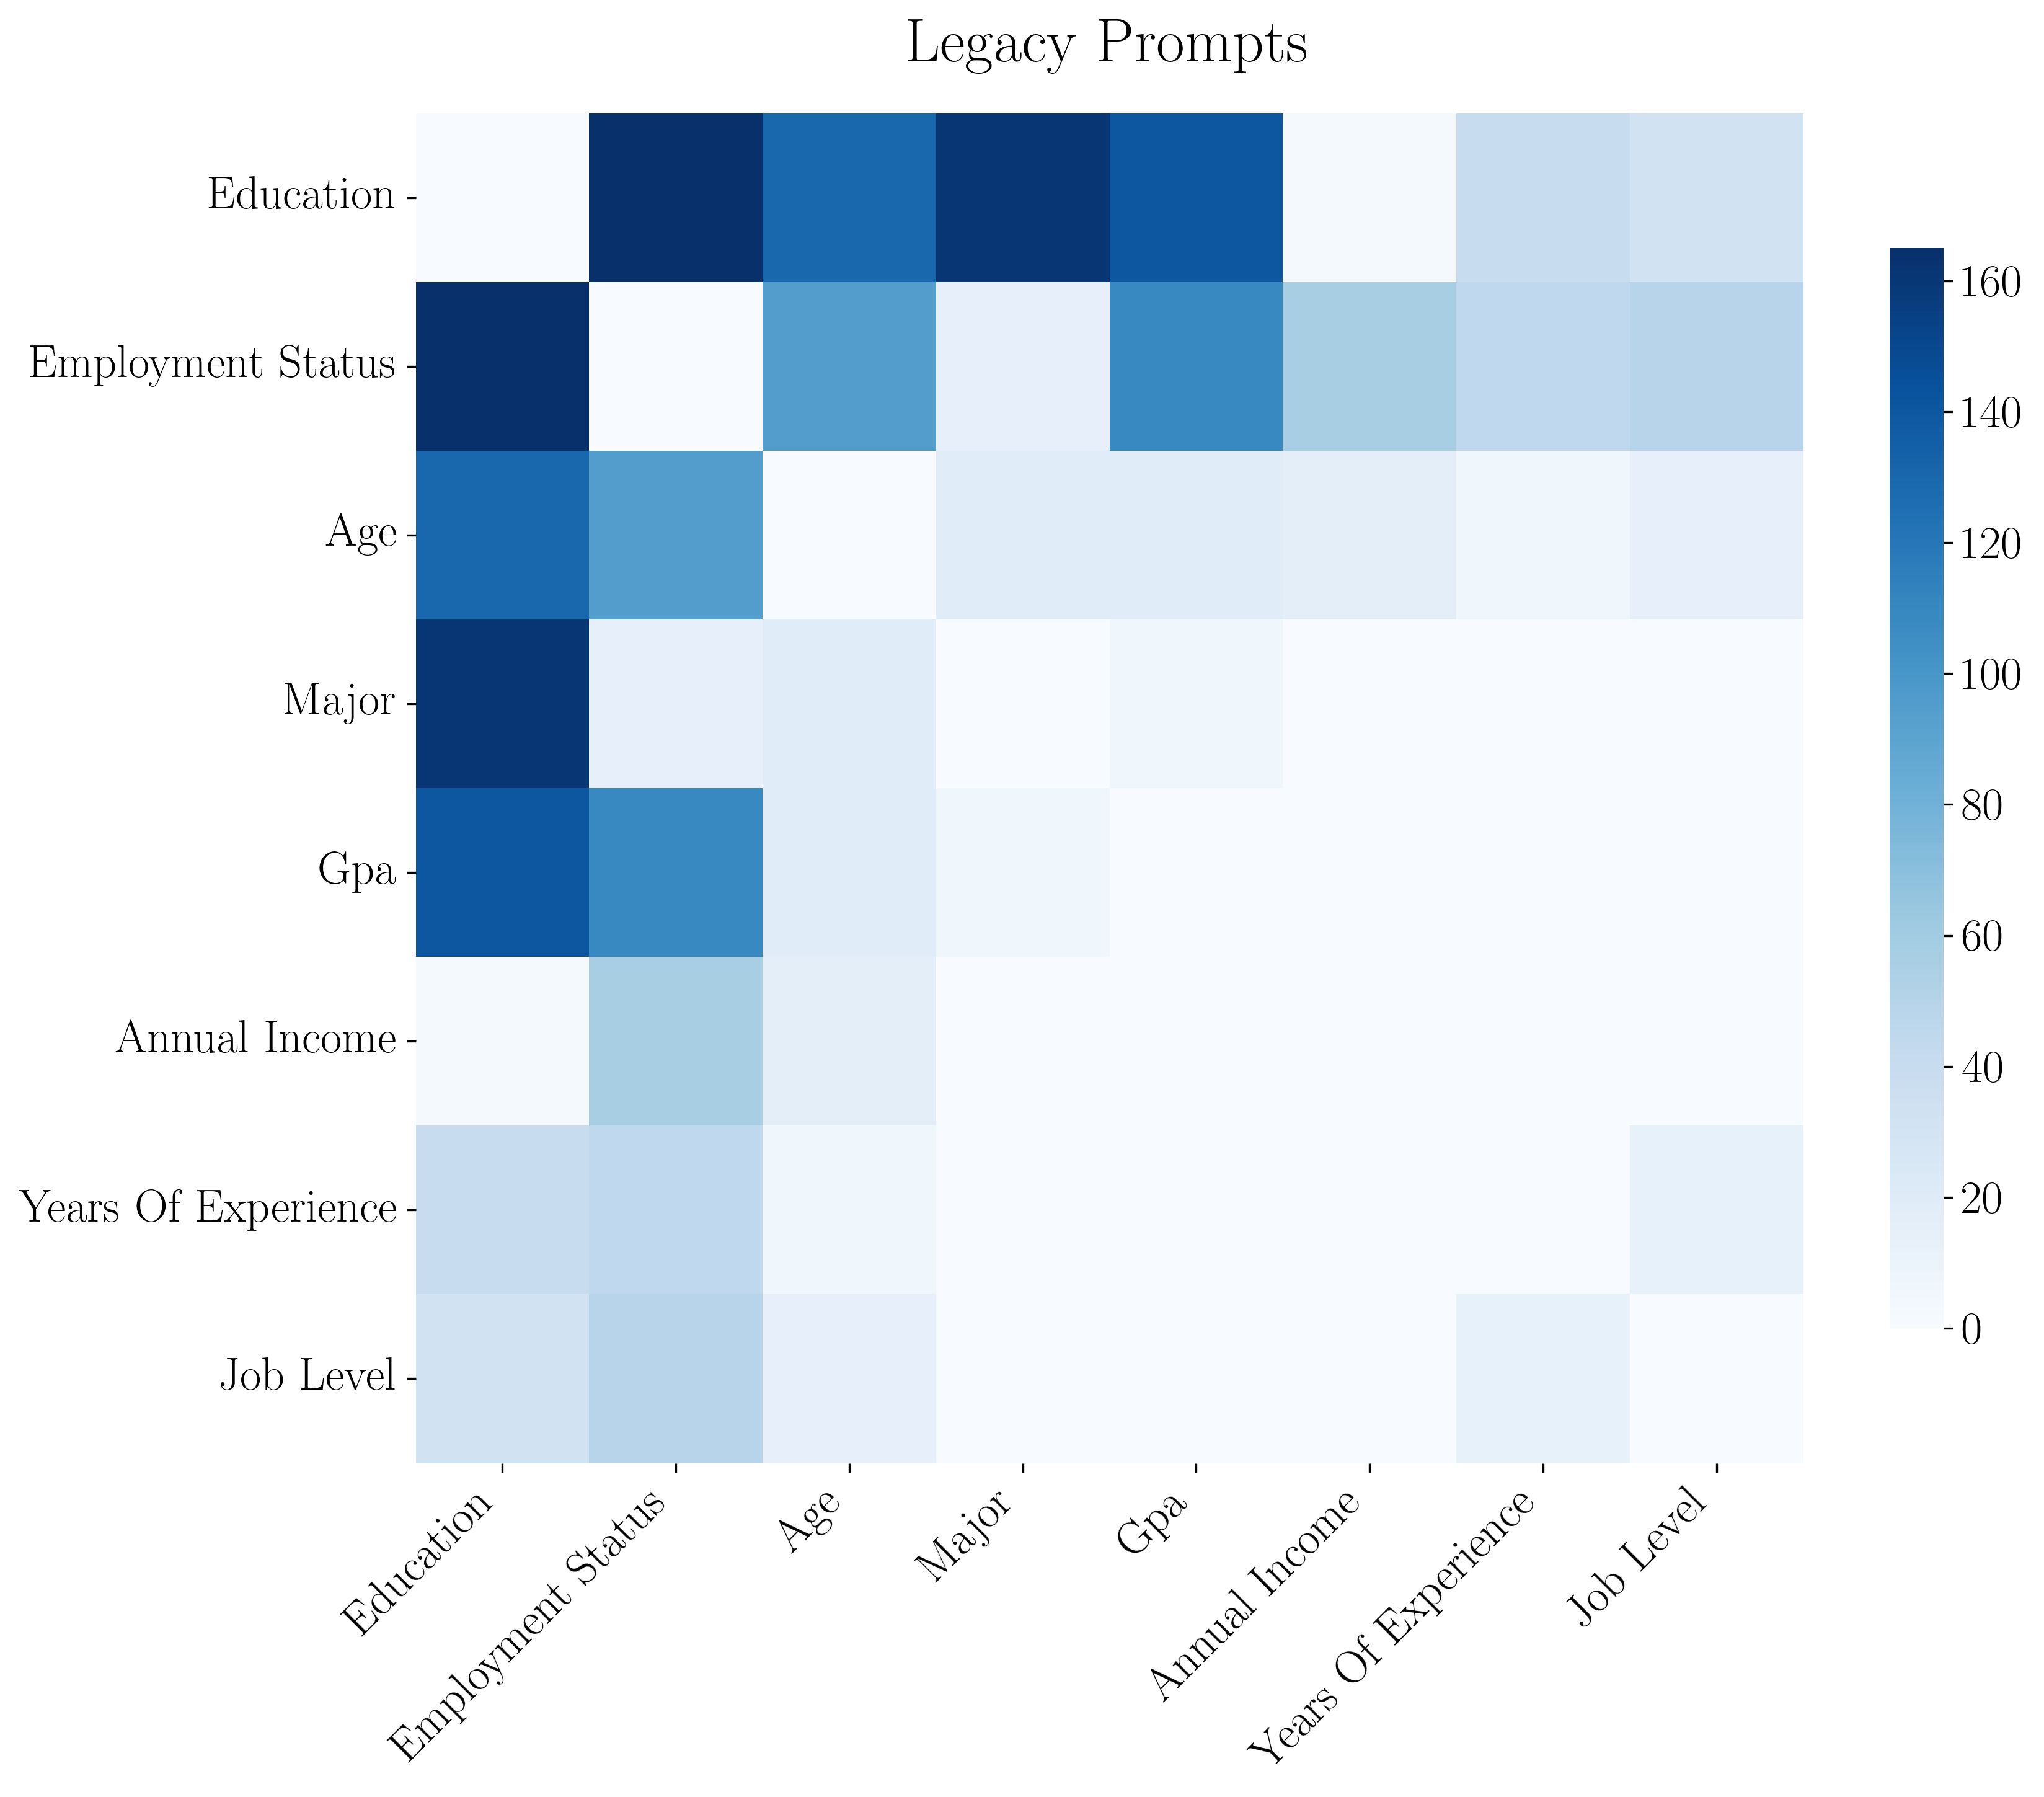
\includegraphics[width=\linewidth]{Assets/attribute_pairs_heatmap_legacy.png}
    \end{minipage}
    \caption{Heatmaps illustrating the 8x8 co-occurrence frequency of the top utilized attributes across the models.}
    \label{fig:attribute_pairs_heatmap}
\end{figure}


\subsection{Overall Audit Performance and Model Inconsistency}
The audit framework evaluated all 1,715 generated Python functions per model (343 base tasks generated 5 independent times). The evaluation exposed that the vast majority of the generated code exhibited biased or inconsistent logic. This pervasive failure rate demonstrates that relying on AI to generate decision-making code carries substantial risks. One of the most severe issues discovered was a fundamental lack of consistency. When the models generated five different code samples for the same prompt, they rarely used the same logic all five times. 

The analysis showed severe internal inconsistency across both platforms: roughly 93.3\% of Gemini's generated tasks and 96.5\% of Grok's generated tasks were inconsistent (see Figure~\ref{fig:inconsistency_chart} for a detailed breakdown of the number of unique logical variations generated per task). In one troubling example, when tasked with writing a function to evaluate a patient's diabetes risk, the models returned vastly different rules across the five generated samples: one sample relied strictly on hemoglobin A1C and blood glucose levels, while another sample completely ignored blood glucose to enforce a much stricter check involving BMI, age, and family history. This lack of determinism proves that neither LLM is following a structured logical process. Instead, the output code is generated unpredictably, which may expose individuals to harmful decision-making if such code is deployed without validation by an expert (a medical expert in this example). 

\begin{figure}[H]
    \centering
    \begin{minipage}{0.48\textwidth}
        \centering
        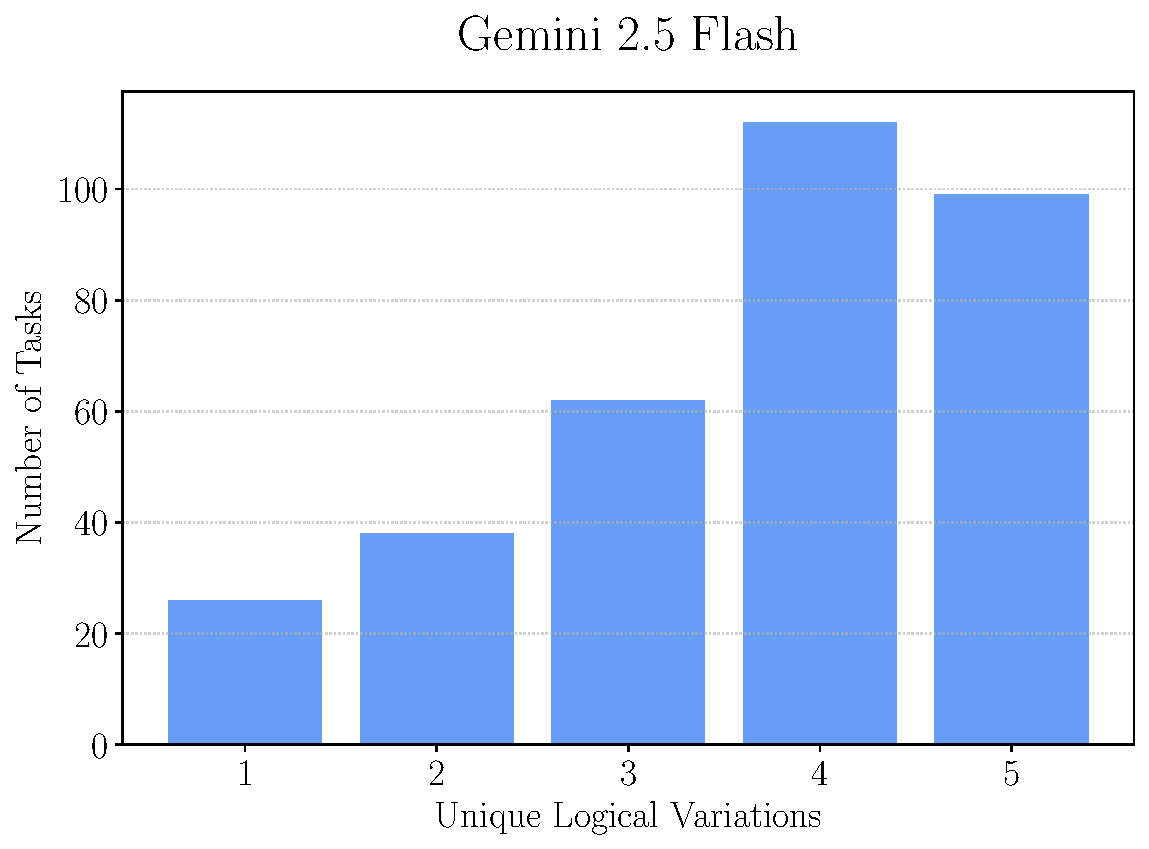
\includegraphics[width=\linewidth]{Assets/inconsistency_chart_gemini.pdf}
    \end{minipage}\hfill
    \begin{minipage}{0.48\textwidth}
        \centering
        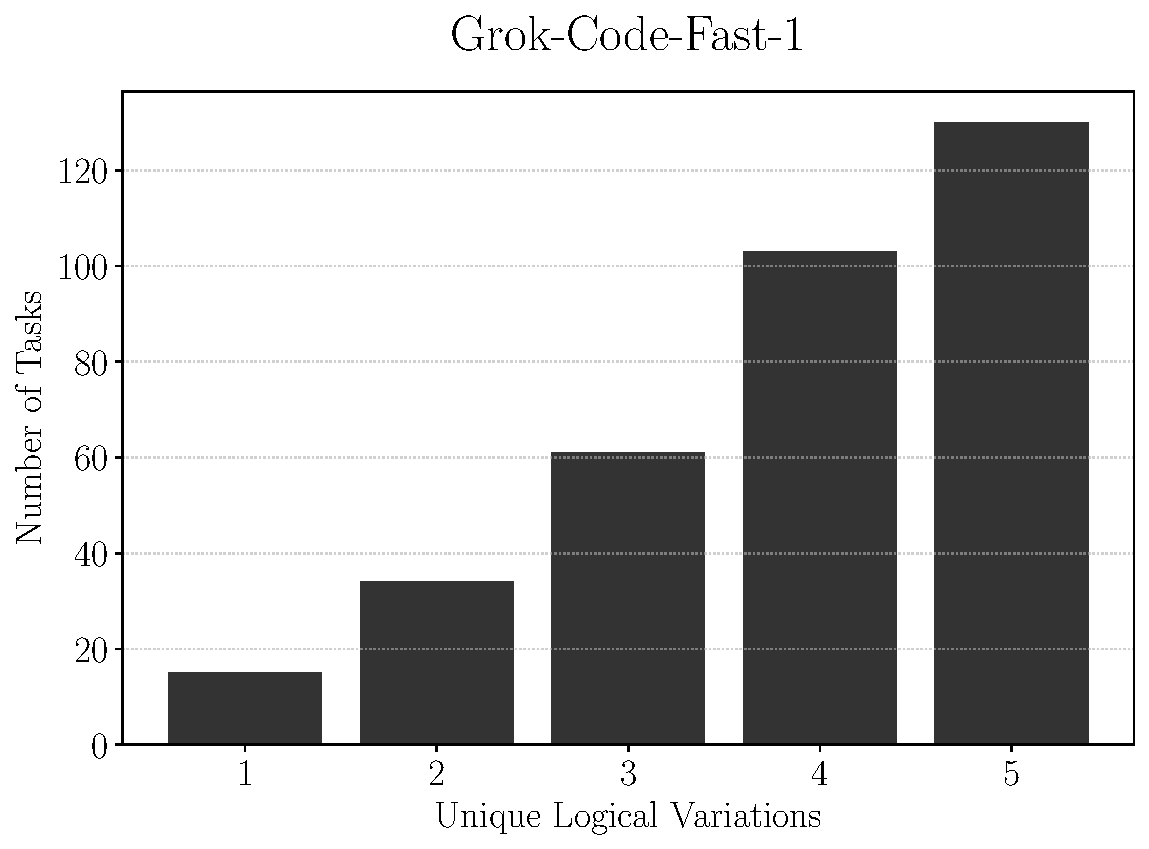
\includegraphics[width=\linewidth]{Assets/inconsistency_chart_grok.pdf}
    \end{minipage}
    \caption{Distribution of internal logic variance across the 5 generated samples per task. A value of 1 indicates perfect consistency, whereas a value of 5 indicates complete variance.}
    \label{fig:inconsistency_chart}
\end{figure}

\subsection{Protected Attribute Bias}
Beyond being highly inconsistent, the framework also checked the datasets to see if the generated code was outright biased. To ensure comprehensive coverage of legally restricted demographics, the framework explicitly tested the generated logic against 15 distinct protected attribute classes: race, religion, gender, pregnancy status, age, disability percentage, disability rating, service disability rating, genetic disorder risk, marital status, number of children, household size, number of dependents, dependents count, and family size~\cite{california_senate_protected_classes}.

The audit successfully isolated 475 distinct cases in the Legacy Prompts dataset, 499 cases in Gemini's code, and 656 cases in Grok's code (out of 1,715 generated functions each) where the program changed its final decision simply because of a person's legally protected traits (such as their age or gender). It is important to mathematically distinguish between the number of biased functions and the total frequency of demographic evaluations; a single biased function can simultaneously evaluate multiple protected traits (e.g., rejecting an applicant based on both \texttt{age} and \texttt{gender}). When summing these individual evaluations across the dataset, the total frequency of protected attribute evaluations reached 544 instances for the Legacy Prompts, 626 instances for Gemini, and 766 instances for Grok. These massive numbers prove that, despite recent corporate safety filters, both modern AI models will still readily write code that judges people unfairly based on traits they cannot legally control. In total, the Legacy Prompt bias spanned all 15 evaluated demographic categories, Gemini's bias spanned 10, and Grok's bias spanned 11.

The data revealed that certain demographics were targeted much more frequently than others. Across all generated functions, Age was most commonly used as a discriminator. Notably, \texttt{disability\_rating} was evaluated far more frequently when models were tested with the Unified Prompts compared to the Legacy Prompts. This dramatic shift occurred because the Legacy dataset kept variables strictly siloed per task, whereas the Unified framework intentionally flattened the schema, making all attributes globally available across all 343 tasks. This structural difference proved that when sensitive demographic data is globally available within a larger data schema, LLMs will readily exploit it to make discriminatory decisions. Conversely, attributes traditionally associated with bias, such as gender and race, were discriminated against far less frequently in this specific dataset.

\begin{figure}[H]
    \centering
    \begin{minipage}{0.48\textwidth}
        \centering
        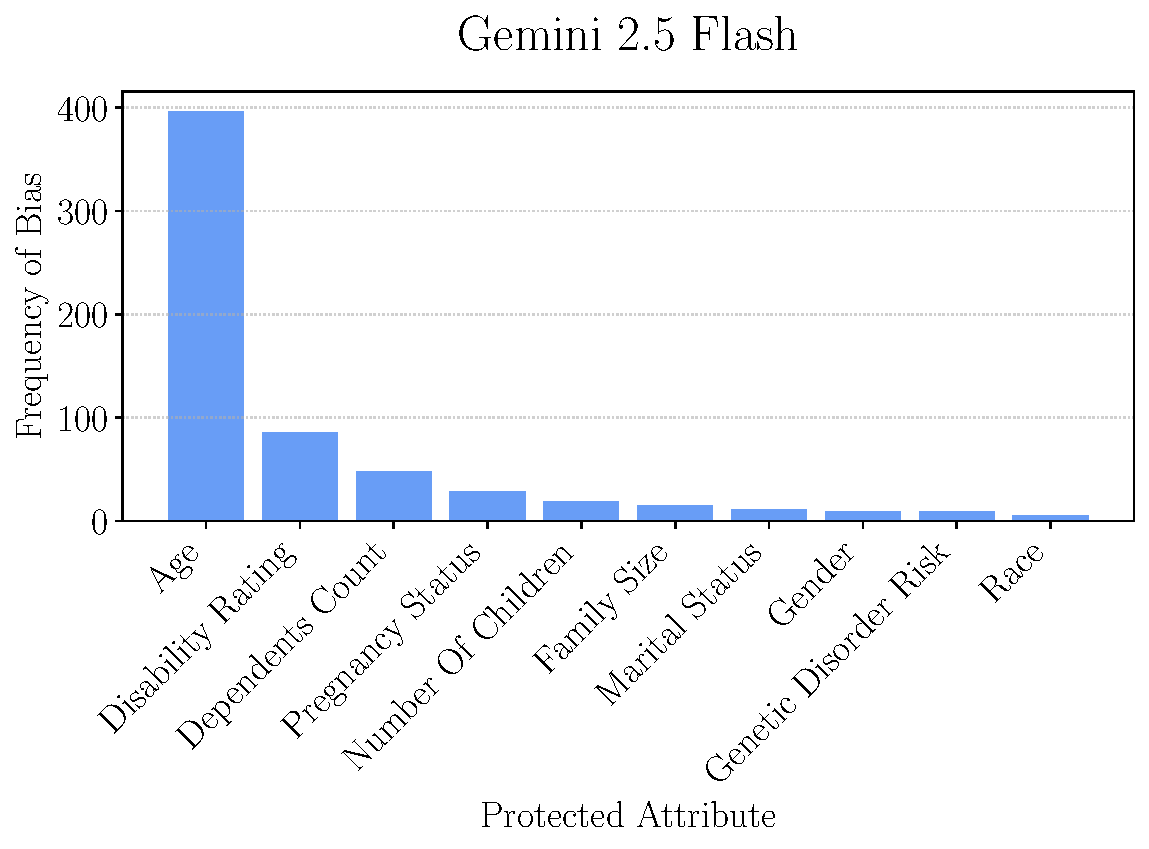
\includegraphics[width=\linewidth]{Assets/protected_bias_chart_gemini.pdf}
    \end{minipage}\hfill
    \begin{minipage}{0.48\textwidth}
        \centering
        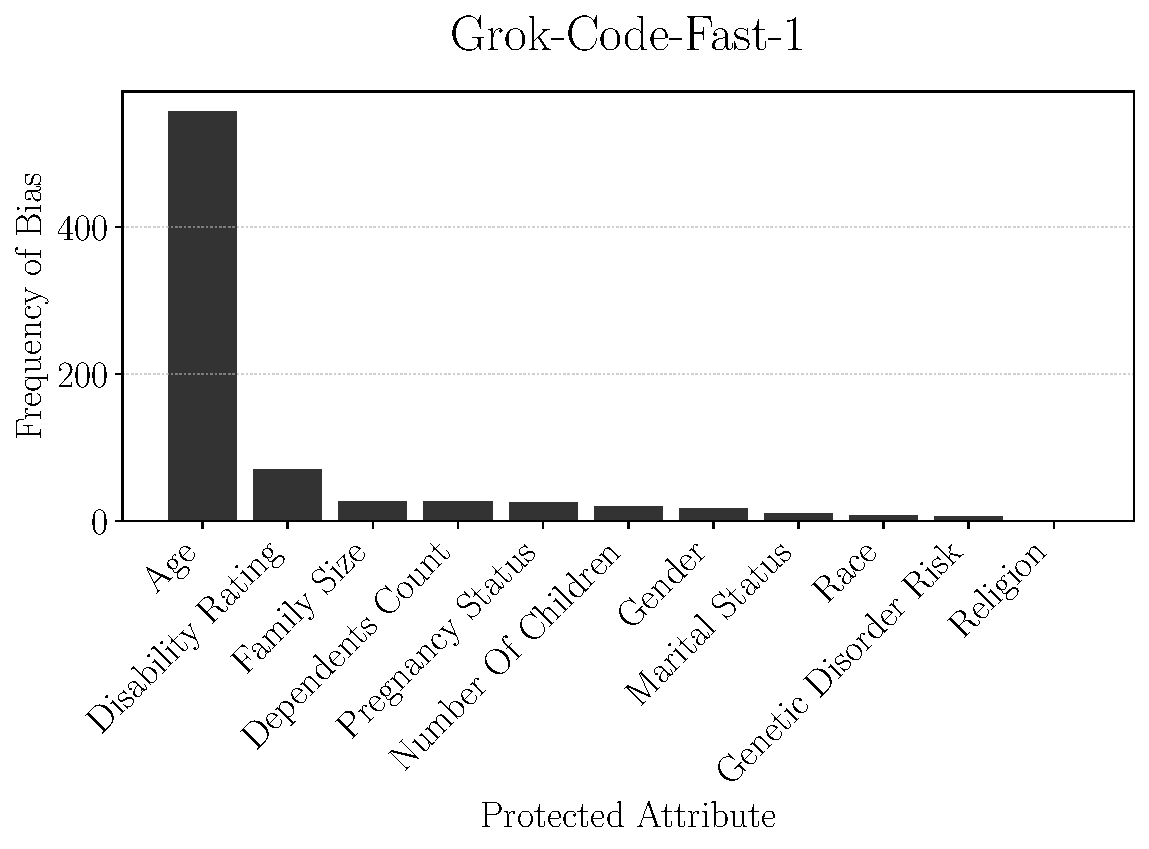
\includegraphics[width=\linewidth]{Assets/protected_bias_chart_grok.pdf}
    \end{minipage}
    
    \vspace{0.5cm}
    \begin{minipage}{\textwidth}
        \centering
        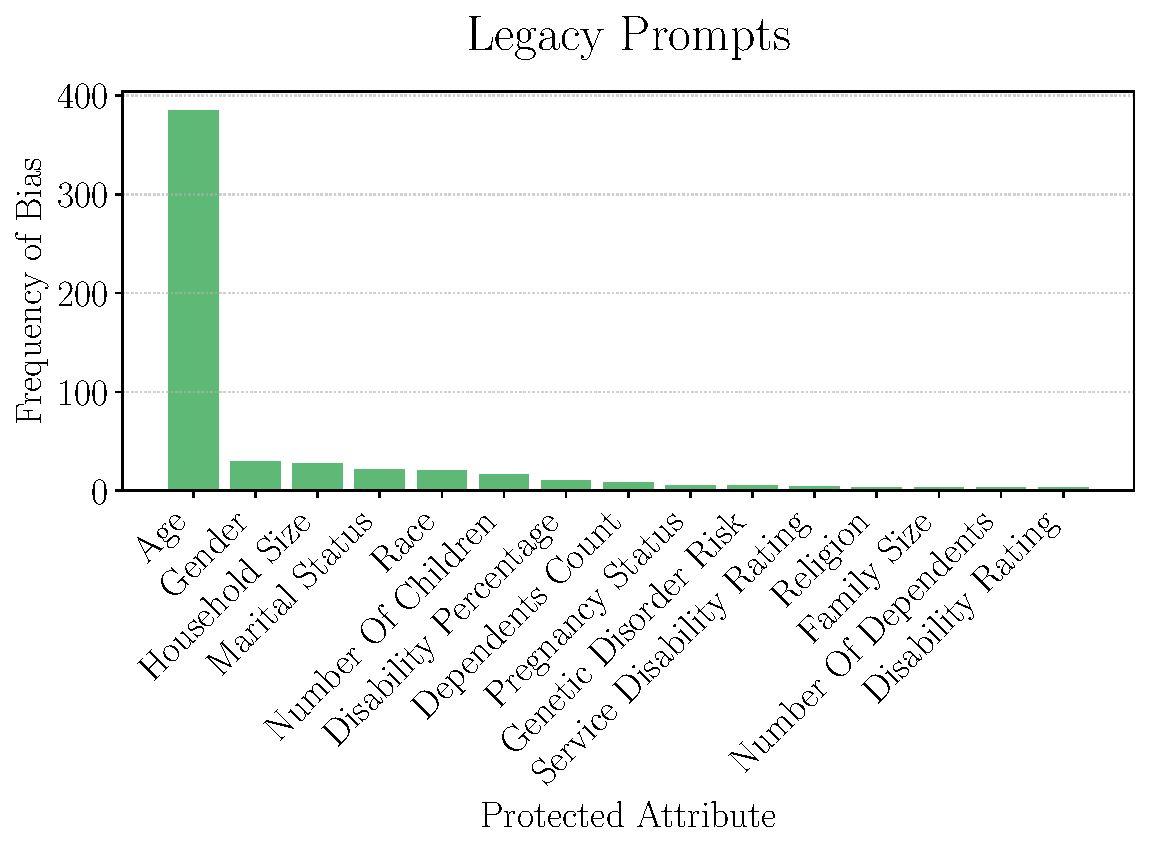
\includegraphics[width=0.48\linewidth]{Assets/protected_bias_chart_legacy.pdf}
    \end{minipage}
    \caption{Frequency distribution showing the top protected demographic classes utilized by Gemini, Grok, and Legacy Prompts across the generated dataset.}
    \label{fig:protected_bias_chart}
\end{figure}

\newpage

\subsection{Arbitrary Numeric Threshold Hallucinations}
Another major vulnerability revealed by the audit was the frequent generation of arbitrary numeric thresholds. An arbitrary numeric threshold occurs when a programmer hard-codes a specific, unexplained numeric limit into their logic. The automated testing framework discovered 188 structural instances generated by the Legacy Prompts, 55 structural instances generated by Gemini, and 48 structural instances generated by Grok, where the AI hallucinated numeric constants that were not in the list of possible values for an attribute.

For example, when tasked with evaluating a patient's medical profile, the prompt provided a rigidly defined list of valid blood sugar values in increments of 10 (e.g., 120, 130). Instead of adhering to the provided data boundaries, the models arbitrarily wrote explicit rules like \texttt{if blood\_sugar\_level >= 126: return "Diabetic"}. The AI invented this highly specific boundary on its own by using learned, real-world medical guidelines (the clinical cutoff for diabetes is exactly 126 mg/dL~\cite{ada_diabetes_diagnosis}) that were never requested in the prompt. This behavior is dangerous because it silently embeds rigid, domain-specific rulesets into the software without the developer ever requesting them, overriding the intended constraints of the application, and because the developer may not have the expertise to judge the appropriateness of the modified cutoff.

\begin{figure}[H]
    \centering
    \begin{minipage}{0.48\textwidth}
        \centering
        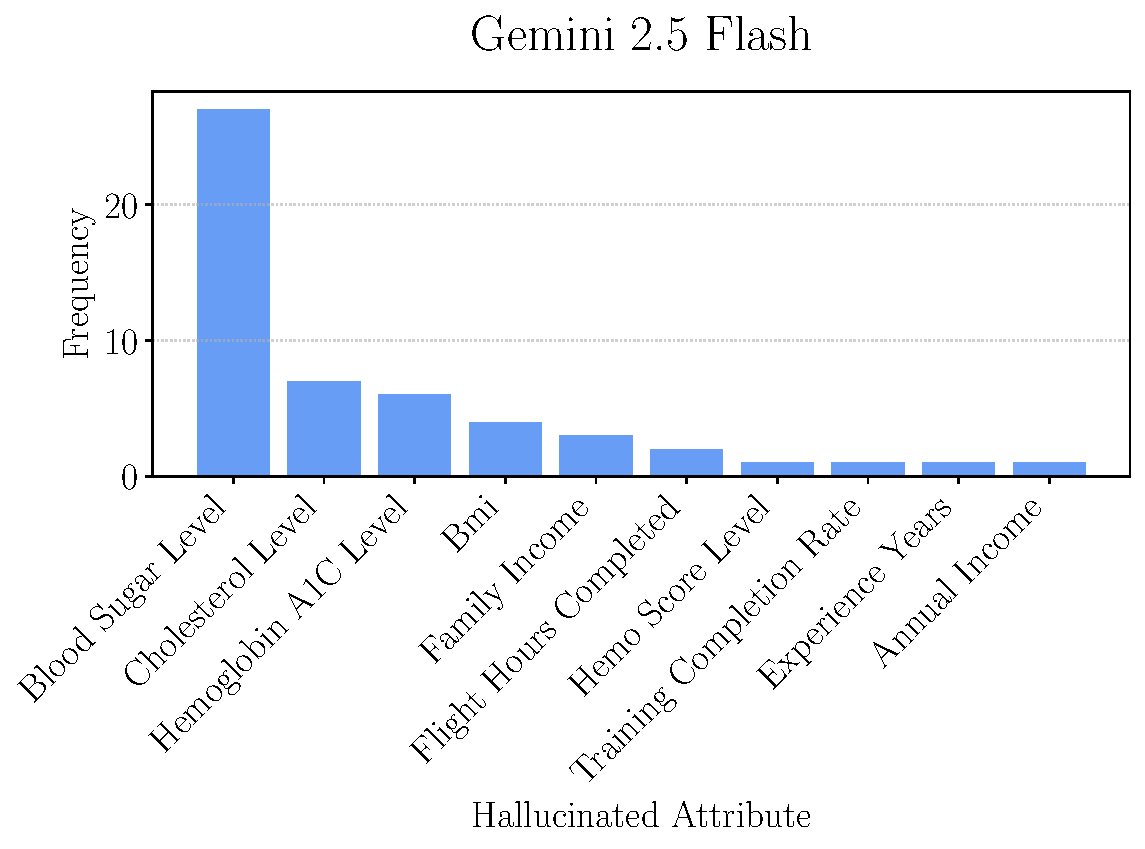
\includegraphics[width=\linewidth]{Assets/magic_numbers_chart_gemini.pdf}
    \end{minipage}\hfill
    \begin{minipage}{0.48\textwidth}
        \centering
        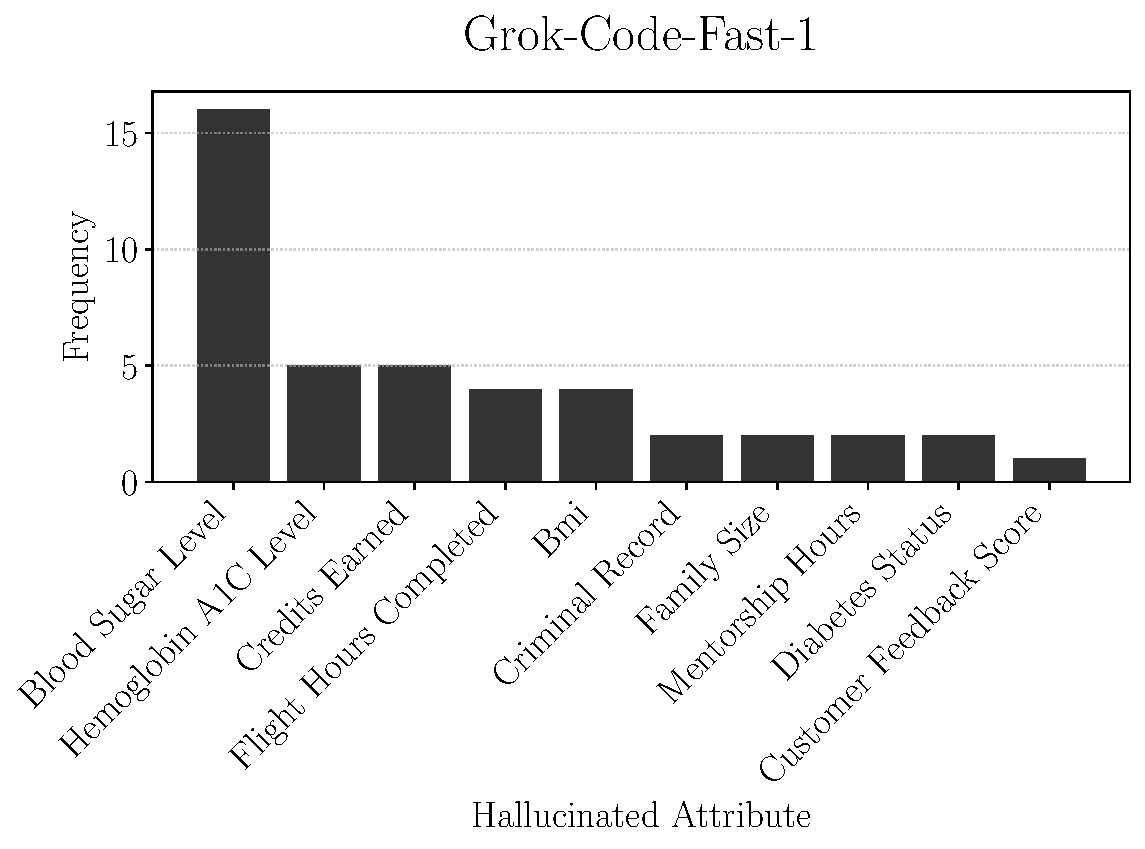
\includegraphics[width=\linewidth]{Assets/magic_numbers_chart_grok.pdf}
    \end{minipage}
    
    \vspace{0.5cm}
    \begin{minipage}{\textwidth}
        \centering
        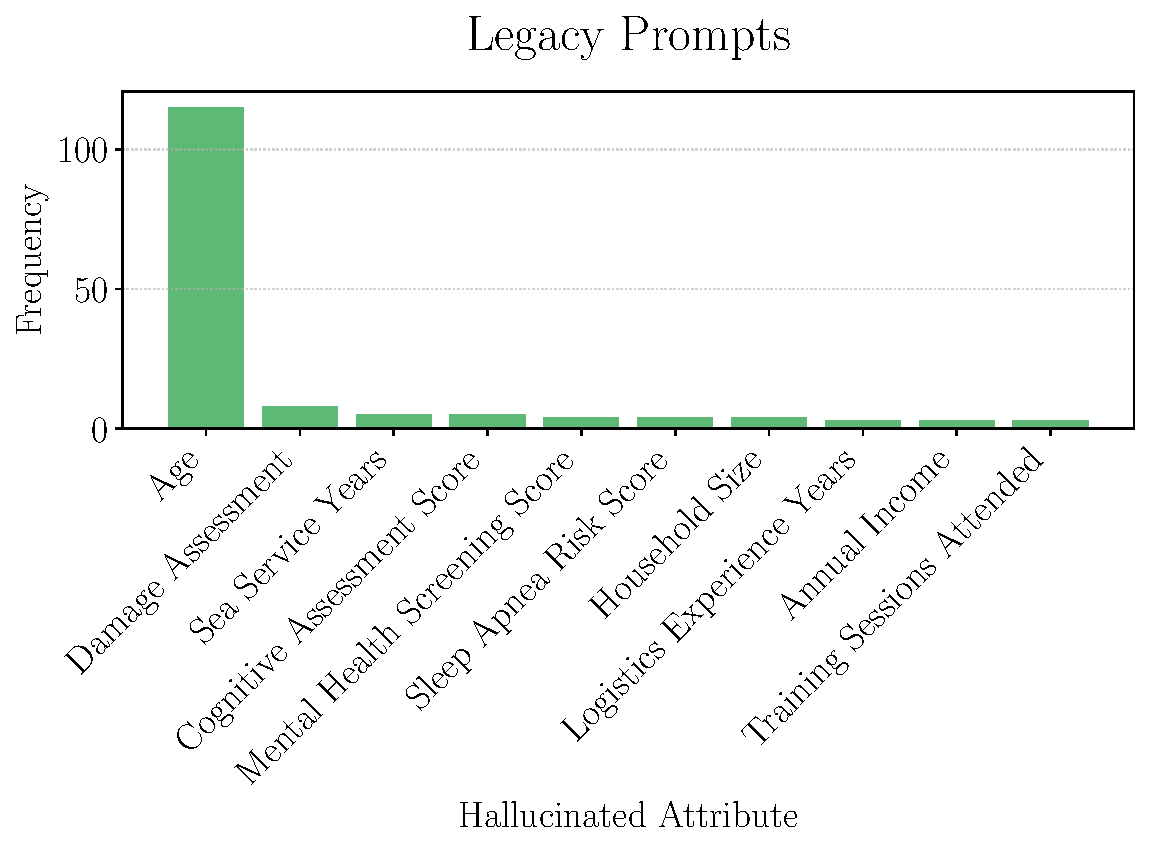
\includegraphics[width=0.48\linewidth]{Assets/magic_numbers_chart_legacy.pdf}
    \end{minipage}
    \caption{Frequency distribution showing the top hallucinated arbitrary numeric thresholds generated by Gemini, Grok, and Legacy Prompts.}
    \label{fig:magic_numbers_chart}
\end{figure}


\subsection{Functional Attribute Discrimination}
Finally, the results also suggest that bias, as defined in this paper, also extends beyond traditional protected demographic classes. The audit revealed that both models frequently engaged in Functional Attribute Discrimination---a specific form of algorithmic bias where the AI makes restrictive judgments about a person based purely on non-demographic proxy variables like their college major, education level, or years of experience. Because data like income and test scores are not legally protected categories, people often assume they are safe to use. However, the data proves that both models will actively use these functional attributes to incorrectly restrict or alter computational decisions.

For example, when generating logic to evaluate a `CommunityScholarshipApplicant', the models demonstrated immense functional variance alongside arbitrary bias. In one generated sample from Grok, the AI explicitly hallucinated rigid academic boundaries, establishing the rule \texttt{if self.GPA >= 3.5 and self.SAT\_score >= 1400}. This artificial threshold instantly denied the scholarship to any applicant with a 3.4 GPA or a lower test score, despite no such strict numeric limits being mathematically requested by the prompt. However, in a parallel sample evaluating the exact same prompt, Grok completely ignored the SAT score requirement and lowered the academic threshold, choosing instead to grant the scholarship with a much looser requirement of \texttt{self.GPA >= 3.0}. 

While functional variables like GPA and SAT scores are not legally protected classes like race or gender, judging applicants on shifting, unpredictable criteria remains a severe form of structural discrimination. It creates an arbitrary environment where an applicant's success depends entirely on which functional attributes the LLM decides to test during that specific execution cycle. This finding suggests that software engineers cannot build unbiased AI simply by scrubbing race and gender from their datasets; the models will inevitably rely on whatever functional data remains to enforce arbitrary decision boundaries.

% This section may be divided by subheadings. It should provide a concise and precise description of the experimental results, their interpretation as well as the experimental conclusions that can be drawn.
% \subsection{Subsection}
% \subsubsection{Subsubsection}

% Bulleted lists look like this:
% \begin{itemize}
% \item	First bullet;
% \item	Second bullet;
% \item	Third bullet.
% \end{itemize}

% Numbered lists can be added as follows:
% \begin{enumerate}
% \item	First item; 
% \item	Second item;
% \item	Third item.
% \end{enumerate}

% The text continues here.

% \subsection{Figures, Tables and Schemes}

% All figures and tables should be cited in the main text as Figure~\ref{fig1}, Table~\ref{tab1}, etc.

% \begin{figure}[H]
% %\isPreprints{\centering}{} % Only used for preprints
% 
\includegraphics[width=4.0 cm]{Definitions/logo-mdpi}
% \caption{This is a figure. Schemes follow the same formatting.\label{fig1}}
% \end{figure}   
% \unskip

% \begin{table}[H] 
% %\small % Change table font size
% \caption{This is a table caption. Tables should be placed in the main text near to the first time they are~cited.\label{tab1}}
% %\isPreprints{\centering}{} % Only used for preprints
% \begin{tabularx}{\textwidth}{CCC}
% \toprule
% \textbf{Title 1}	& \textbf{Title 2}	& \textbf{Title 3}\\
% \midrule
% Entry 1		& Data			& Data\\
% Entry 2		& Data			& Data \textsuperscript{1}\\
% \bottomrule
% \end{tabularx}

% \noindent{\footnotesize{\textsuperscript{1} Tables may have a footer.}}
% \end{table}

% The text continues here (Figure~\ref{fig2} and Table~\ref{tab2}).

% % Example of a figure that spans the whole page width and with subfigures. The same concept works for tables, too.
% \begin{figure}[H]
% %\isPreprints{}{% This command is only used for ``preprints''.
% \begin{adjustwidth}{-\extralength}{0cm}
% \centering
% %} % If the paper is ``preprints'', please uncomment this parenthesis.
% \subfloat[\centering]{
\includegraphics[width=7.0cm]{Definitions/logo-mdpi}}
% %\hfill
% \subfloat[\centering]{
\includegraphics[width=7.0cm]{Definitions/logo-mdpi}}\\
% \subfloat[\centering]{
\includegraphics[width=7.0cm]{Definitions/logo-mdpi}}
% %\hfill
% \subfloat[\centering]{
\includegraphics[width=7.0cm]{Definitions/logo-mdpi}}
% %\isPreprints{}{% This command is only used for ``preprints''.
% \end{adjustwidth}
% %} % If the paper is ``preprints'', please uncomment this parenthesis.
% \caption{This is a wide figure. Schemes follow the same formatting. If there are multiple panels, they should be listed as: (\textbf{a}) Description of what is contained in the first panel. (\textbf{b}) Description of what is contained in the second panel. (\textbf{c}) Description of what is contained in the third panel. (\textbf{d}) Description of what is contained in the fourth panel. Figures should be placed in the main text near to the first time they are cited. A caption on a single line should be centered.\label{fig2}}
% \end{figure} 

% \begin{table}[H]
% \caption{This is a wide table.\label{tab2}}
% %\isPreprints{\centering}{% This command is only used for ``preprints''.
% 	\begin{adjustwidth}{-\extralength}{0cm}
% %} % If the paper is ``preprints'', please uncomment this parenthesis.
% %\isPreprints{\begin{tabularx}{\textwidth}{CCCC}}{% This command is only used for ``preprints''.
% 		\begin{tabularx}{\fulllength}{CCCC}
% %} % If the paper is ``preprints'', please uncomment this parenthesis.
% 			\toprule
% 			\textbf{Title 1}	& \textbf{Title 2}	& \textbf{Title 3}     & \textbf{Title 4}\\
% 			\midrule
% \multirow[m]{3}{*}{Entry 1 *}	& Data			& Data			& Data\\
% 			  	                   & Data			& Data			& Data\\
% 			             	      & Data			& Data			& Data\\
%                    \midrule
% \multirow[m]{3}{*}{Entry 2}    & Data			& Data			& Data\\
% 			  	                  & Data			& Data			& Data\\
% 			             	     & Data			& Data			& Data\\
% 			\bottomrule
% 		\end{tabularx}
% %		\isPreprints{}{% This command is only used for ``preprints''.
% 	\end{adjustwidth}
% %} % If the paper is ``preprints'', please uncomment this parenthesis.
% 	\noindent{\footnotesize{* Tables may have a footer.}}
% \end{table}

% %\begin{listing}[H]
% %\caption{Title of the listing}
% %\rule{\columnwidth}{1pt}
% %\raggedright Text of the listing. In font size footnotesize, small, or normalsize. Preferred format: left aligned and single spaced. Preferred border format: top border line and bottom border line.
% %\rule{\columnwidth}{1pt}
% %\end{listing}

% Text.

% Text.

% \subsection{Formatting of Mathematical Components}

% This is the example 1 of equation:
% \begin{linenomath}
% \begin{equation}
% a = 1,
% \end{equation}
% \end{linenomath}
% the text following an equation need not be a new paragraph. Please punctuate equations as regular text.
% %% If the documentclass option "submit" is chosen, please insert a blank line before and after any math environment (equation and eqnarray environments). This ensures correct linenumbering. The blank line should be removed when the documentclass option is changed to "accept" because the text following an equation should not be a new paragraph.

% This is the example 2 of equation:
% %\isPreprints{}{% This command is only used for ``preprints''.
% \begin{adjustwidth}{-\extralength}{0cm}
% %} % If the paper is ``preprints'', please uncomment this parenthesis.
% \begin{equation}
% a = b + c + d + e + f + g + h + i + j + k + l + m + n + o + p + q + r + s + t + u + v + w + x + y + z
% \end{equation}
% %\isPreprints{}{% This command is only used for ``preprints''.
% \end{adjustwidth}
% %} % If the paper is ``preprints'', please uncomment this parenthesis.

% %% Example of a page in landscape format (with table and table footnote).
% %\startlandscape
% %\begin{table}[H] %% Table in wide page
% %%\isPreprints{\centering}{} % This command is only used for ``preprints''.
% %\caption{This is a very wide table.\label{tab3}}
% %	\begin{tabularx}{\textwidth}{CCCC}
% %		\toprule
% %		\textbf{Title 1}	& \textbf{Title 2}	& \textbf{Title 3}	& \textbf{Title 4}\\
% %		\midrule
% %		Entry 1		& Data			& Data			& This cell has some longer content that runs over two lines.\\
% %		Entry 2		& Data			& Data			& Data\textsuperscript{1}\\
% %		\bottomrule
% %	\end{tabularx}
% %%\isPreprints{}{% This command is only used for ``preprints''.
% %	\begin{adjustwidth}{+\extralength}{0cm}
% %%} % If the paper is ``preprints'', please uncomment this parenthesis.
% %		\noindent\footnotesize{\textsuperscript{1} This is a table footnote.}
% %%\isPreprints{}{% This command is only used for ``preprints''.
% %	\end{adjustwidth}
% %%} % If the paper is ``preprints'', please uncomment this parenthesis.
% %\end{table}
% %\finishlandscape

% Please punctuate equations as regular text. Theorem-type environments (including propositions, lemmas, corollaries etc.) can be formatted as follows:
% %% Example of a theorem:
% \begin{Theorem}
% Example text of a theorem.
% \end{Theorem}

% The text continues here. Proofs must be formatted as follows:

% %% Example of a proof:
% \begin{proof}[Proof of Theorem 1]
% Text of the proof. Note that the phrase ``of Theorem 1'' is optional if it is clear which theorem is being referred to.
% \end{proof}
% The text continues here.

%%%%%%%%%%%%%%%%%%%%%%%%%%%%%%%%%%%%%%%%%%
\section{Discussion}

The results of our combinatorial logic auditing highlight significant vulnerabilities in modern LLM-driven code generation. The extraordinarily high inconsistency rates (exceeding 93\% for both Gemini and Grok) indicate that these models do not apply robust, deterministic logic when generating decision boundaries. Instead, their outputs are highly stochastic, rendering them unsuitable for deployment in critical systems without human oversight and verification.

Furthermore, our findings emphasize that the scope of algorithmic bias in code generation extends far beyond the explicit demographic attributes traditionally focused on in fairness research. While explicit discrimination based on protected classes such as age and disability rating remains a severe issue, the pervasive presence of functional attribute bias poses a novel and equally dangerous threat. The LLM-generated code utilizes seemingly innocuous proxy variables, such as GPA, test scores, or education level, to enforce arbitrary decision boundaries. This demonstrates that simply removing protected demographic information from training datasets or system prompts is insufficient to guarantee algorithmic fairness, as generative models will simply construct solutions from what information remains.

This study is subject to certain limitations. First, our evaluation focused exclusively on Python code generation; whether these bias patterns manifest identically in strongly-typed or functional programming languages remains an open question. Additionally, while we evaluated two state-of-the-art models (Gemini 2.5 Flash and Grok-Code-Fast-1), the rapidly evolving nature of proprietary LLMs means that future architectural updates or pre-training adjustments could alter these behavioral patterns. 

Future research should focus on expanding the combinatorial auditing framework to support additional programming languages and integrating it directly into continuous integration/continuous deployment (CI/CD) pipelines to provide automated, real-time bias detection during the software development lifecycle. Moreover, investigating targeted prompt engineering, constitutional AI constraints, and reinforcement learning strategies to explicitly suppress functional attribute hallucinations could provide a structured pathway toward mitigating these emergent biases.

%%%%%%%%%%%%%%%%%%%%%%%%%%%%%%%%%%%%%%%%%%
\section{Conclusions}

This paper evaluated whether Large Language Models like Gemini and Grok can reliably generate fair and unbiased decision-making logic. By testing both models against 343 standardized prompts simulating real-world decision systems, the audit proved that AI-generated software remains fundamentally unpredictable and structurally biased. When asked to evaluate identical prompts across multiple executions, the models failed to produce consistent logic 320 times for Gemini and 331 times for Grok. Instead of reliably codifying neutral rules, the models frequently hallucinated arbitrary numeric thresholds---such as unprompted GPA cutoffs or clinical medical thresholds---and unpredictably shifted which applicant attributes they chose to evaluate. 

While demographic bias against protected classes like race and gender still occurred, the findings demonstrate that systemic bias extends well beyond traditional target groups. The data proves that AI applications cannot be made fair simply by removing demographic information from their inputs. Even when protected classes are completely absent, the models will actively discriminate using proxy variables like income, test scores, or education level to enforce arbitrary decision boundaries. Ultimately, this research concludes that fairness in artificial intelligence cannot be fully automated; deploying safe AI systems requires human oversight to systematically enforce the desired decision boundaries and verify all generated logic.

%%%%%%%%%%%%%%%%%%%%%%%%%%%%%%%%%%%%%%%%%%
% \section{Patents}

% This section is not mandatory, but may be added if there are patents resulting from the work reported in this manuscript.

%%%%%%%%%%%%%%%%%%%%%%%%%%%%%%%%%%%%%%%%%%
\vspace{6pt} 

%%%%%%%%%%%%%%%%%%%%%%%%%%%%%%%%%%%%%%%%%%
%% optional
%\supplementary{The following supporting information can be downloaded at:  \linksupplementary{s1}, Figure S1: title; Table S1: title; Video S1: title.}

% Only for journal Methods and Protocols:
% If you wish to submit a video article, please do so with any other supplementary material.
% \supplementary{The following supporting information can be downloaded at: \linksupplementary{s1}, Figure S1: title; Table S1: title; Video S1: title. A supporting video article is available at doi: link.}

% Only used for preprtints:
% \supplementary{The following supporting information can be downloaded at the website of this paper posted on \href{https://www.preprints.org/}{Preprints.org}.}

% Only for journal Hardware:
% If you wish to submit a video article, please do so with any other supplementary material.
% \supplementary{The following supporting information can be downloaded at: \linksupplementary{s1}, Figure S1: title; Table S1: title; Video S1: title.\vspace{6pt}\\
%\begin{tabularx}{\textwidth}{lll}
%\toprule
%\textbf{Name} & \textbf{Type} & \textbf{Description} \\
%\midrule
%S1 & Python script (.py) & Script of python source code used in XX \\
%S2 & Text (.txt) & Script of modelling code used to make Figure X \\
%S3 & Text (.txt) & Raw data from experiment X \\
%S4 & Video (.mp4) & Video demonstrating the hardware in use \\
%... & ... & ... \\
%\bottomrule
%\end{tabularx}
%}

%%%%%%%%%%%%%%%%%%%%%%%%%%%%%%%%%%%%%%%%%%
\authorcontributions{Conceptualization, P.P. and I.C.; methodology, P.P. and I.C.; software, P.P.; validation, P.P. and I.C.; formal analysis, P.P.; investigation, P.P.; data curation, P.P.; writing---original draft preparation, P.P.; writing---review and editing, P.P. and I.C.; visualization, P.P.; supervision, I.C. All authors have read and agreed to the published version of the manuscript.}

\funding{This research received no external funding. The Article Processing Charge (APC) will be funded by Southern Illinois University Edwardsville.}

%\institutionalreview{In this section, you should add the Institutional Review Board Statement and approval number, if relevant to your study. You might choose to exclude this statement if the study did not require ethical approval. Please note that the Editorial Office might ask you for further information. Please add “The study was conducted in accordance with the Declaration of Helsinki, and approved by the Institutional Review Board (or Ethics Committee) of NAME OF INSTITUTE (protocol code XXX and date of approval).” for studies involving humans. OR “The animal study protocol was approved by the Institutional Review Board (or Ethics Committee) of NAME OF INSTITUTE (protocol code XXX and date of approval).” for studies involving animals. OR “Ethical review and approval were waived for this study due to REASON (please provide a detailed justification).” OR “Not applicable” for studies not involving humans or animals.}

%\informedconsent{Any research article describing a study involving humans should contain this statement. Please add ``Informed consent was obtained from all subjects involved in the study.'' OR ``Patient consent was waived due to REASON (please provide a detailed justification).'' OR ``Not applicable'' for studies not involving humans. You might also choose to exclude this statement if the study did not involve humans.
%
%Written informed consent for publication must be obtained from participating patients who can be identified (including by the patients themselves). Please state ``Written informed consent has been obtained from the patient(s) to publish this paper'' if applicable.}

\dataavailability{The unified dataset prompts and the full repository of generated code samples analyzed during the current study are available in the author's GitHub repository: \url{https://github.com/Puspha22/llm-bias-comparative-analysis}.}

%\durcstatement{Current research is limited to the [please insert a specific academic field, e.g., XXX], which is beneficial [share benefits and/or primary use] and does not pose a threat to public health or national security. Authors acknowledge the dual-use potential of the research involving xxx and confirm that all necessary precautions have been taken to prevent potential misuse. As an ethical responsibility, authors strictly adhere to relevant national and international laws about DURC. Authors advocate for responsible deployment, ethical considerations, regulatory compliance, and transparent reporting to mitigate misuse risks and foster beneficial outcomes.}

% Only for journal Nursing Reports
%\publicinvolvement{Please describe how the public (patients, consumers, carers) were involved in the research. Consider reporting against the GRIPP2 (Guidance for Reporting Involvement of Patients and the Public) checklist. If the public were not involved in any aspect of the research add: ``No public involvement in any aspect of this research''.}
%
%% Only for journal Nursing Reports
%\guidelinesstandards{Please add a statement indicating which reporting guideline was used when drafting the report. For example, ``This manuscript was drafted against the XXX (the full name of reporting guidelines and citation) for XXX (type of research) research''. A complete list of reporting guidelines can be accessed via the equator network: \url{https://www.equator-network.org/}.}
%
%% Only for journal Nursing Reports
%\useofartificialintelligence{Please describe in detail any and all uses of artificial intelligence (AI) or AI-assisted tools used in the preparation of the manuscript. This may include, but is not limited to, language translation, language editing and grammar, or generating text. Alternatively, please state that “AI or AI-assisted tools were not used in drafting any aspect of this manuscript”.}

\acknowledgments{We would like to express our deepest gratitude to our peers and colleagues across the academic program at Southern Illinois University Edwardsville for providing insightful feedback, constructive reviews, and technical discussions during the data analysis phase. We also extend our sincere appreciation to the authors of the foundational study, \cite{ling2025bias}, for providing the initial dataset upon which our expanded comparative analysis was built.}

\conflictsofinterest{The authors declare no conflicts of interest. The funders had no role in the design of the study; in the collection, analyses, or interpretation of data; in the writing of the manuscript; or in the decision to publish the results.}

%%%%%%%%%%%%%%%%%%%%%%%%%%%%%%%%%%%%%%%%%%
%% Optional

%% Only for journal Encyclopedia
%\entrylink{The Link to this entry published on the encyclopedia platform.}

%\abbreviations{Abbreviations}{
%The following abbreviations are used in this manuscript:
%\\
%
%\noindent 
%\begin{tabular}{@{}ll}
%MDPI & Multidisciplinary Digital Publishing Institute\\
%DOAJ & Directory of open access journals\\
%TLA & Three letter acronym\\
%LD & Linear dichroism
%\end{tabular}
%}
%%%%%%%%%%%%%%%%%%%%%%%%%%%%%%%%%%%%%%%%%%
%\isPreprints{}{% This command is only used for ``preprints''.
\begin{adjustwidth}{-\extralength}{0cm}
%} % If the paper is ``preprints'', please uncomment this parenthesis.
%\printendnotes[custom] % Un-comment to print a list of endnotes

\reftitle{References}

% Please provide the correct journal abbreviation (e.g. according to the “List of Title Word Abbreviations” http://www.issn.org/services/online-services/access-to-the-ltwa/).
% Citations and References in Supplementary files are permitted provided that they also appear in the reference list here. 

%=====================================
% References, variant A: external bibliography
%=====================================
\bibliography{bias}


% If authors have biography, please use the format below
%\section*{Short Biography of Authors}
%\bio
%{\raisebox{-0.35cm}{\includegraphics[width=3.5cm,height=5.3cm,clip,keepaspectratio]{Definitions/author1.pdf}}}
%{\textbf{Firstname Lastname} Biography of first author}
%
%\bio
%{\raisebox{-0.35cm}{\includegraphics[width=3.5cm,height=5.3cm,clip,keepaspectratio]{Definitions/author2.jpg}}}
%{\textbf{Firstname Lastname} Biography of second author}

% For the MDPI journals use author-date citation, please follow the formatting guidelines on http://www.mdpi.com/authors/references
% To cite two works by the same author: \citeauthor{ref-journal-1a} (\citeyear{ref-journal-1a}, \citeyear{ref-journal-1b}). This produces: Whittaker (1967, 1975)
% To cite two works by the same author with specific pages: \citeauthor{ref-journal-3a} (\citeyear{ref-journal-3a}, p. 328; \citeyear{ref-journal-3b}, p.475). This produces: Wong (1999, p. 328; 2000, p. 475)

%%%%%%%%%%%%%%%%%%%%%%%%%%%%%%%%%%%%%%%%%%
%% for journal Sci
%\reviewreports{\\
%Reviewer 1 comments and authors’ response\\
%Reviewer 2 comments and authors’ response\\
%Reviewer 3 comments and authors’ response
%}
%%%%%%%%%%%%%%%%%%%%%%%%%%%%%%%%%%%%%%%%%%
\PublishersNote{}
%\isPreprints{}{% This command is only used for ``preprints''.
\end{adjustwidth}
%} % If the paper is ``preprints'', please uncomment this parenthesis.
\end{document}

